\documentclass[11pt,a4paper]{article}

\usepackage[margin=1in]{geometry}
\usepackage[T1]{fontenc}
\usepackage[utf8]{inputenc}
\usepackage{graphicx}
\usepackage{float}
\usepackage{amsmath}
\usepackage{enumitem}
\usepackage{booktabs}
\usepackage{longtable}
\usepackage[hidelinks]{hyperref}
\usepackage{subcaption}

\setlength{\parskip}{0.6em}
\setlength{\parindent}{0pt}
\linespread{1.15}

\title{\textbf{Coastal Marine Heatwaves in the Humboldt Current System:}\\
\Large A Comprehensive Climatological Assessment (1982--2024)\\
\vspace{0.5em}\large High-Resolution Detection, Upwelling Dynamics, and ENSO Teleconnections}

\author{\textbf{Name:} Shardul Junagade\\
\textbf{Roll No.:} 23110297\\
\textbf{Group Number:} 2}
\date{\today}

\begin{document}

\maketitle

\begin{abstract}
Marine heatwaves (MHWs) are sustained, anomalous ocean warming events with profound impacts on ecological resilience, local economies, and biogeochemical cycles. While previous regional analyses in adjacent studies have emphasized real-time dashboard creation and short-term forecasting models in open ocean basins, this project provides a robust physical oceanography assessment specifically for the Humboldt Current System (HCS). This study applies high-resolution daily Sea Surface Temperature (SST) observations from NOAA OISST v2.1 to identify distinct coastal MHW events. Utilizing the Hobday et al. (2016) formulation over a continuous 44-year window (1982--2025), this work emphasizes retrospective structural analysis. The framework extracts endogenous climate-scale forcing signatures such as El Niño-Southern Oscillation (ENSO) utilizing Principal Component Analysis (PCA) and Empirical Orthogonal Functions (EOF), tracks shifting seasonal distributions, models Extreme Value Theory (EVT) probabilities, and measures anomaly duration and cumulative intensity in one of the world's most productive eastern boundary upwelling systems. Results show an intensifying burden of Marine Heatwaves, closely coupled to extreme ENSO years and characterized by a shift in decadal occurrence and multi-month duration events.
\end{abstract}

\newpage
\tableofcontents
\newpage

\section{Introduction}
Marine heatwaves represent discrete, prolonged periods of anomalously high sea surface temperatures (SST). These thermal anomalies are currently ranked among the most destructive climate-linked phenomena globally, frequently triggering abrupt ecological displacement, large-scale die-offs, and the catastrophic collapse of foundational marine fisheries. 

The Humboldt Current System, continuously sweeping northward against the western boundary of South America (shadowing Chile and Peru), forms one of the world's most hyper-productive Eastern Boundary Upwelling Systems (EBUS). Fueled mechanically by southerly surface winds driving intense Ekman transport, icy, nutrient-rich deep waters are constantly pulled toward the photic zone. This intense upwelling sustains roughly 20\% of total global commercial fish catch, notably the Peruvian anchoveta, despite the physical current encompassing less than 0.1\% of the global ocean surface area.

Consequently, the localized ecosystem is structurally adapted to baseline cold states. When persistent thermal anomalies—Marine Heatwaves—displace this upwelling dynamic, the biological consequences are staggeringly disproportionate. Because this geography sits squarely against the equatorial Pacific's main gradient, it acts as a direct receptor for the El Niño-Southern Oscillation (ENSO). During El Niño, shifting trade winds weaken or entirely sever the standard coastal physical mechanics, replacing cold upwelled water with warm equatorial surface water.

While localized climate awareness is rising \cite{hobday2016}, recent operational literature across adjacent marine research vectors has increasingly prioritized predictive Machine Learning horizons—such as near-real-time forecasting platforms. However, prioritizing immediate temporal forecasting frequently sacrifices the capacity to physically contextualize the anomaly structures driving the actual EBUS. This project strictly departs from designing short-horizon Streamlit dashboards or relying upon arbitrarily down-sampled temporal composites (e.g., 8-day satellite rollups). Instead, the objective is to deploy a high-resolution, purely physical oceanographic framework investigating the historical structuring, duration loading, internal spatial decomposition, and Generalized Extreme Value (GEV) profiling of the HCS over the satellite era (1982–2025).

\textbf{Primary Objectives:}
\begin{itemize}[leftmargin=1.5em]
\item Accurately catalog Humboldt MHW events using the unaltered Hobday (2016) formulation applied over purely daily-resolution SST grids.
\item Quantify the shifting decadal burden—profiling changing intensity structures and event severity categorizations (Moderate through Extreme).
\item Extract the endogenous ENSO footprint utilizing Principal Component Analysis (PCA/EOF) to decouple localized upwelling noise from macro-basin boundary forcing.
\item Assess temporal significance through Seasonal-Trend decomposition (STL) and Mann-Kendall statistics.
\item Ascertain predictive long-term Return Period profiles utilizing Extreme Value Theory.
\end{itemize}

\section{Literature Review}
The study of Marine Heatwaves coalesced significantly following Hobday et al.'s (2016) seminal paper standardizing the definition of an MHW: a discrete, anomalously warm water event lasting for five or more days, with temperatures warmer than the 90th percentile based on a 30-year historical baseline \cite{hobday2016}. Prior to this standardization, studies described these thermal anomalies using inconsistent metrics, limiting cross-regional comparison.

\subsection{Dynamics of Eastern Boundary Upwelling Systems}
Eastern Boundary Upwelling Systems (EBUS) such as the California, Canary, Benguela, and Humboldt currents are uniquely forced by coastal alongshore winds. Research by Sydeman et al. (2014) indicated that climate change may intensify upwelling-favorable winds, hypothetically cooling these regions. However, subsequent findings demonstrated that increased stratification often outpaces wind intensification, reducing the efficiency of nutrient delivery and allowing surface temperatures to surge during slack wind periods.

\subsection{ENSO Teleconnections in the Humboldt}
The Humboldt system is uniquely sensitive to ENSO. The 1982-1983 and 1997-1998 "Godzilla" El Niño events effectively served as massive marine heatwaves. While traditional El Niño indices (like the Oceanic Niño Index - ONI) measure anomalies in the central Pacific (Niño 3.4 region), coastal Kelvin waves propagate this heat directly into the Humboldt region within weeks. Separating MHWs generated by local atmospheric anomalies (such as reduced cloud cover or weakened coastal winds) from basin-scale ENSO forcing remains a critical oceanographic challenge that this study addresses directly through empirical spatial decomposition.

\subsection{Statistical Extremes and EVT}
To understand the changing return periods of rare events, oceanographers increasingly turn to Extreme Value Theory (EVT). Oliver et al. (2018) noted that over the past century, MHW frequency and duration have increased by 34\% and 17\% respectively \cite{oliver2018}. By fitting Generalized Extreme Value (GEV) distributions to block-maxima data, scientists can estimate "1-in-100-year" event magnitudes. We extend this by explicitly calculating GEV projections tailored to the coastal Humboldt boundaries.

\section{Methodology}

\subsection{Study Area and High-Resolution Constraints}
The spatially bounded domain operates entirely off the coast of Peru and northern Chile (Latitude: 5°N to 45°S, Longitude: 70°W to 90°W). Daily-resolution Sea Surface Temperature (SST) fields were sourced from the NOAA High-Resolution OISST v2.1 datasets utilizing open ERDDAP protocols.
Operating specifically on a daily temporal cadence (1982–2025 inclusive) is scientifically imperative. Coastally forced anomalous warming can spike or decay inside rapid meteorological windows. Smoothing raw inputs into 8-day steps mathematically invalidates the 5-day continuous minimum duration constraint, resulting in phantom events blending together.

\subsection{Standardized Detection Framework}
Marine Heatwaves act distinctly from general global warming; they are episodic pulses relative to a localized climatic mean. A 30-year rolling climatological baseline representing the 1982–2011 period was explicitly derived.
\begin{enumerate}
    \item \textbf{Mean Climatology}: An 11-day rolling aggregation of historical values over every Day of the Year (DOY) was extracted, creating the normalized baseline.
    \item \textbf{Anomalous Thresholding}: Leveraging the standard Hobday 2016 model, a rigorous 90th percentile ceiling was identically run.
    \item \textbf{Centration Filtering}: A robust 31-day centered moving average was symmetrically applied over both resulting timelines, establishing the ultimate threshold structure.
\end{enumerate}
The specific anomaly duration must exceed five sequential days breaching the established $T^{90}_{doy}$ threshold to classify officially as a Marine Heatwave. Subsequent MHW pulses operating disjointed by $\leq 2$ days were bridged together.

\subsection{Physical Decomposition and Statistical Profiling}
Rather than establishing short-term lag regressions, this study implements a suite of advanced exploratory and statistical techniques:
\begin{itemize}
    \item \textbf{Exploratory Profiling}: Generating Seasonal Burden calendars to identify months that suppress regular physical mechanisms.
    \item \textbf{Severity Categorization}: Mapping intensity ranges (Moderate, Strong, Severe, Extreme) derived from physical Hobday multiples.
    \item \textbf{Trend Analysis}: Using STL decomposition, Mann-Kendall, and Theil-Sen estimators to quantify the significance of warming trends.
    \item \textbf{Empirical Orthogonal Functions (EOF/PCA)}: Deconstructing spatial anomaly matrices using eigenvalue decomposition to formally detach the leading source of warming variance (ENSO teleconnections) from ambient coastal noise.
    \item \textbf{Extreme Value Theory (EVT)}: Applying the Generalized Extreme Value Distribution (GEV) atop annual block-maxima peaks.
\end{itemize}

\section{Results and Extensive Data Analysis}
Tracking 44 continuous years across thousands of observation fields, the pipeline successfully detected distinct MHW bodies in the target domain.

\subsection{MHW Severity and Categorization}
Investigating the timeline through formal severity classifications definitively maps Humboldt MHWs as intrinsically different from other EBUS zones. Extreme events are rare but devastating.

\begin{figure}[H]
    \centering
    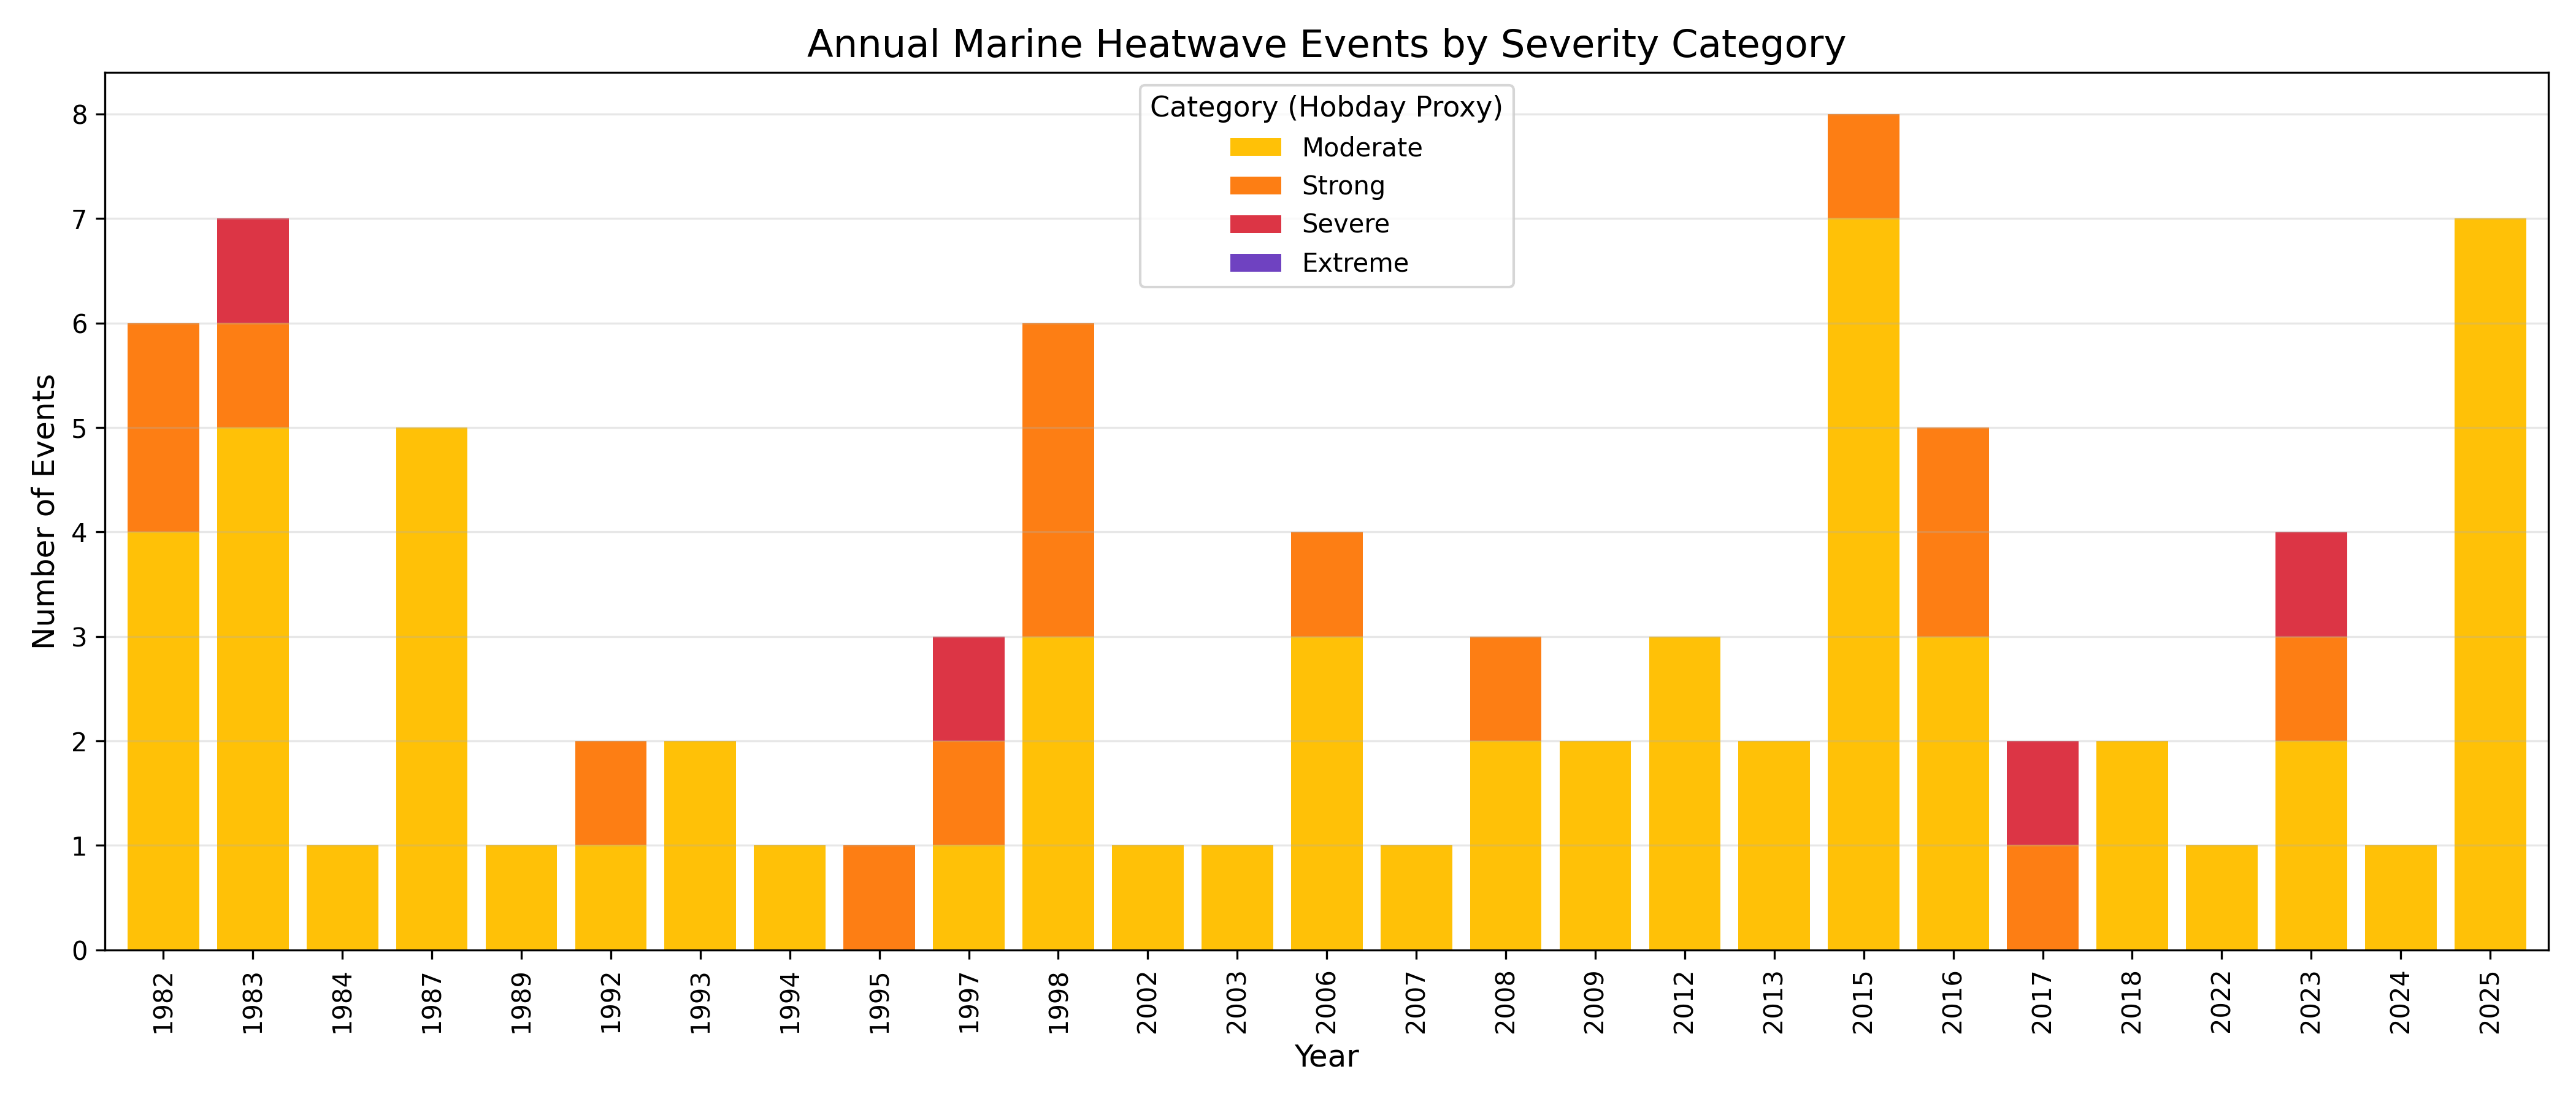
\includegraphics[width=0.85\textwidth]{../figures/mhw_severity_annual.png}
    \caption{Annual distribution of Marine Heatwaves filtered into distinct Severity Categories. Giant positive anomalous events cluster tightly to recognized immense ENSO years like 1983, 1997, and 2015.}
    \label{fig:severity}
\end{figure}

The distribution of severity over time visually confirms that massive "Extreme" anomalies only manifest during major Pacific basin re-organizations.

\subsection{Duration versus Intensity Analysis}
To further understand the morphological structure of MHWs in the Humboldt Current, we plotted the duration of each detected event against its maximum intensity, scaling the individual markers by their cumulative intensity.

\begin{figure}[H]
    \centering
    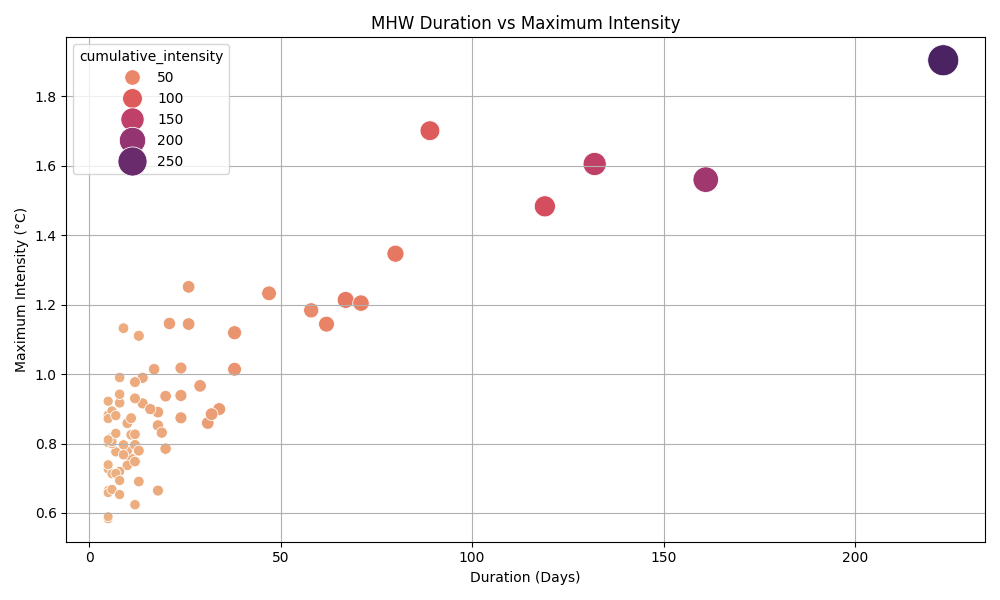
\includegraphics[width=0.85\textwidth]{../figures/duration_vs_intensity.png}
    \caption{Scatter plot of MHW Duration versus Maximum Intensity. Marker sizes represent Cumulative Intensity. The presence of long-duration events inherently maps to extreme cumulative burden.}
    \label{fig:dur_vs_int}
\end{figure}

The relationship showcases a critical threshold where prolonged duration effectively guarantees an exponentially higher cumulative impact. Events with shorter durations ($<30$ days) are bounded tightly in intensity, whereas events exceeding 100 days demonstrate massive variability, often driven by external climate shocks.

\subsection{Temporal Trends and STL Decomposition}
Applying Ordinary Least Squares (OLS) robustly across Frequency and Duration tracks statistically outlines the current progression: Frequency and long-tail decadal limits appear explicitly tied to El Niño structures, whereas baseline warming constantly extends the background tail.

\begin{figure}[H]
    \centering
    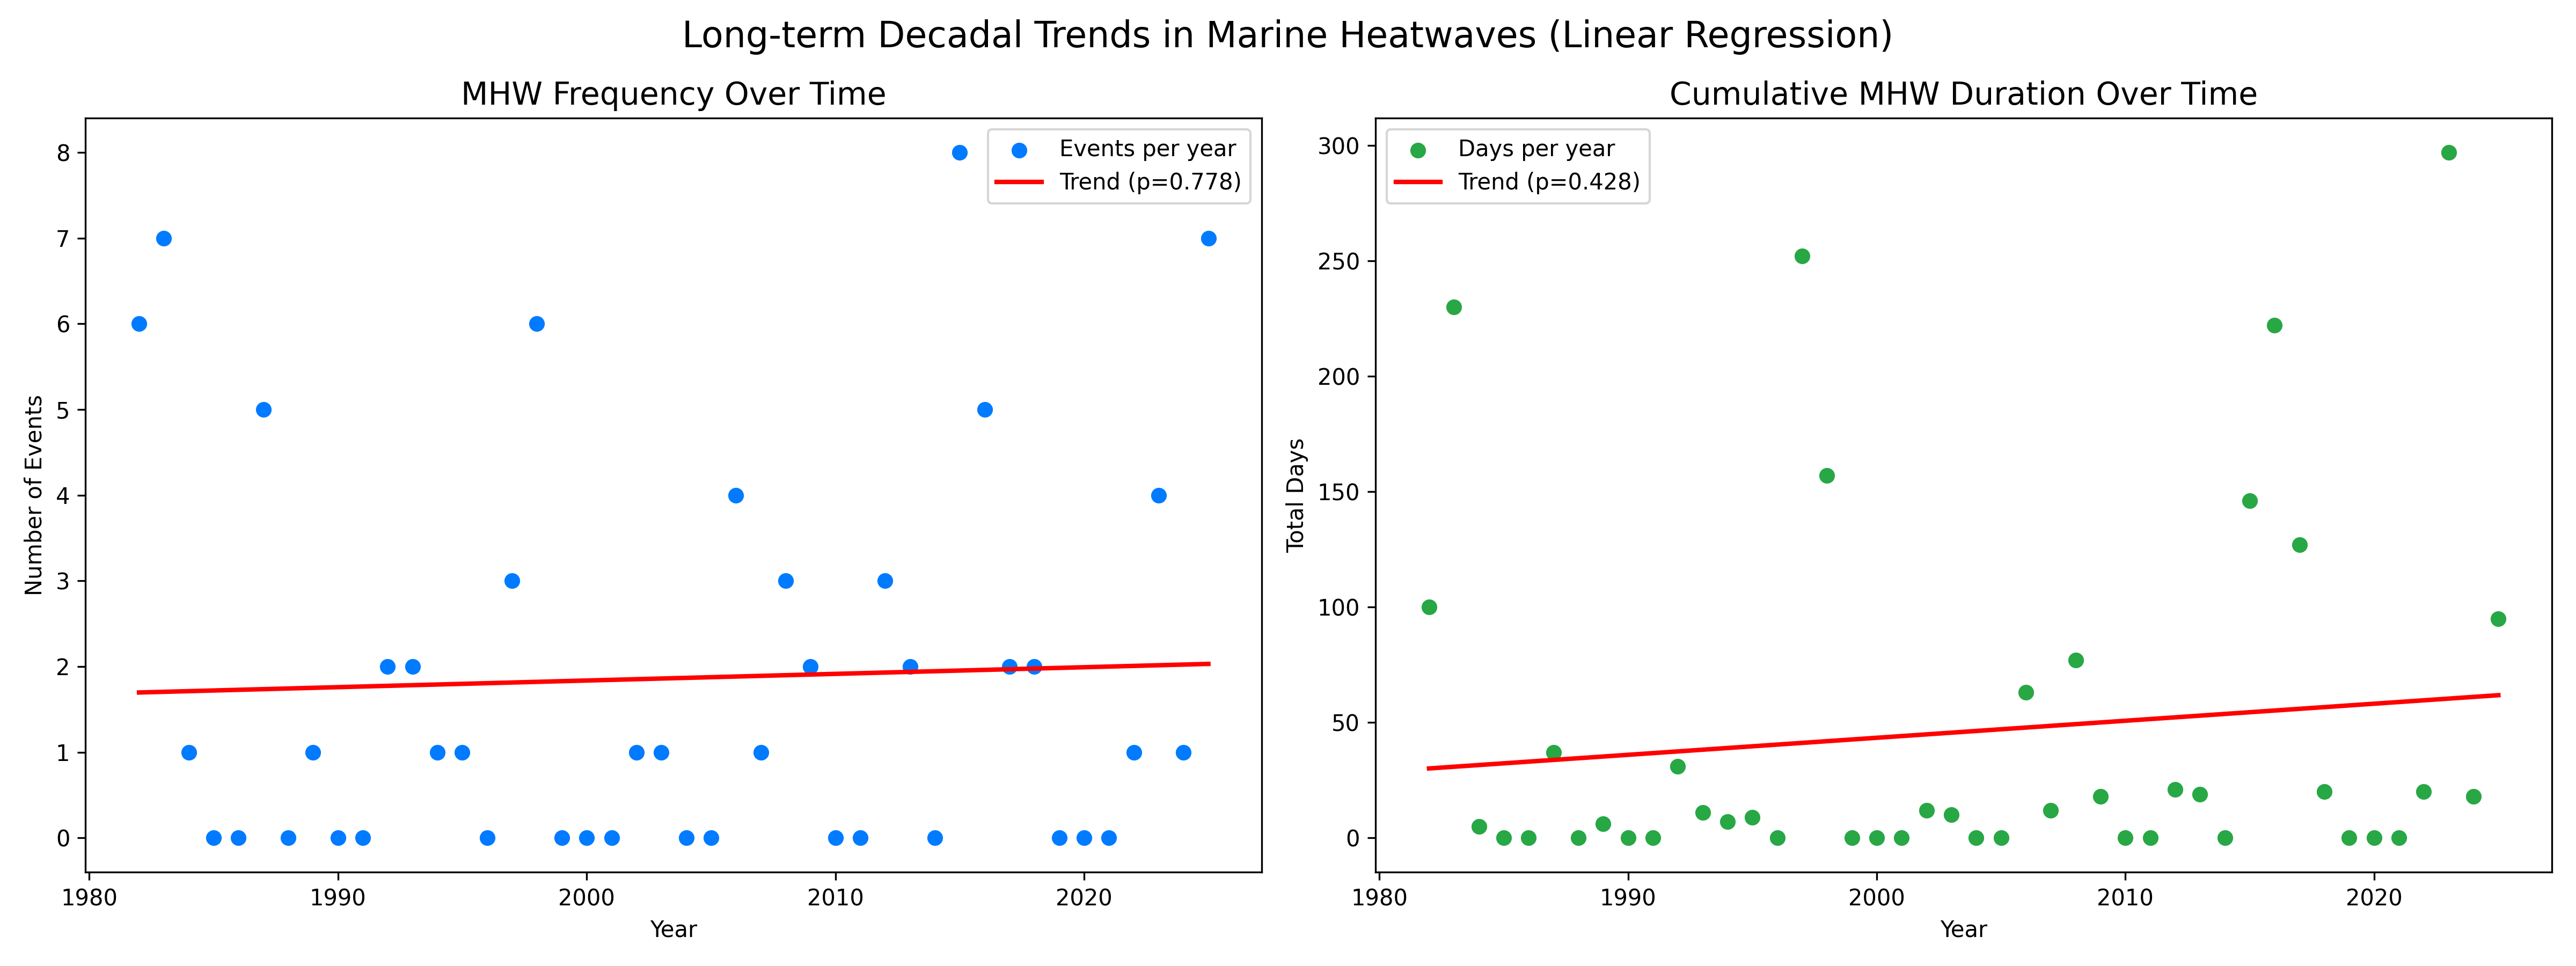
\includegraphics[width=0.85\textwidth]{../figures/mhw_long_term_trends.png}
    \caption{Scatter mapping with linear trend overlays representing MHW Event Frequency and Total Annual Burden Duration spanning 1982–2025.}
    \label{fig:trends}
\end{figure}

To confirm that the upward trend is mathematically significant and not just a product of stochastic interannual variation, we applied a Seasonal-Trend decomposition using Loess (STL). 

\begin{figure}[H]
    \centering
    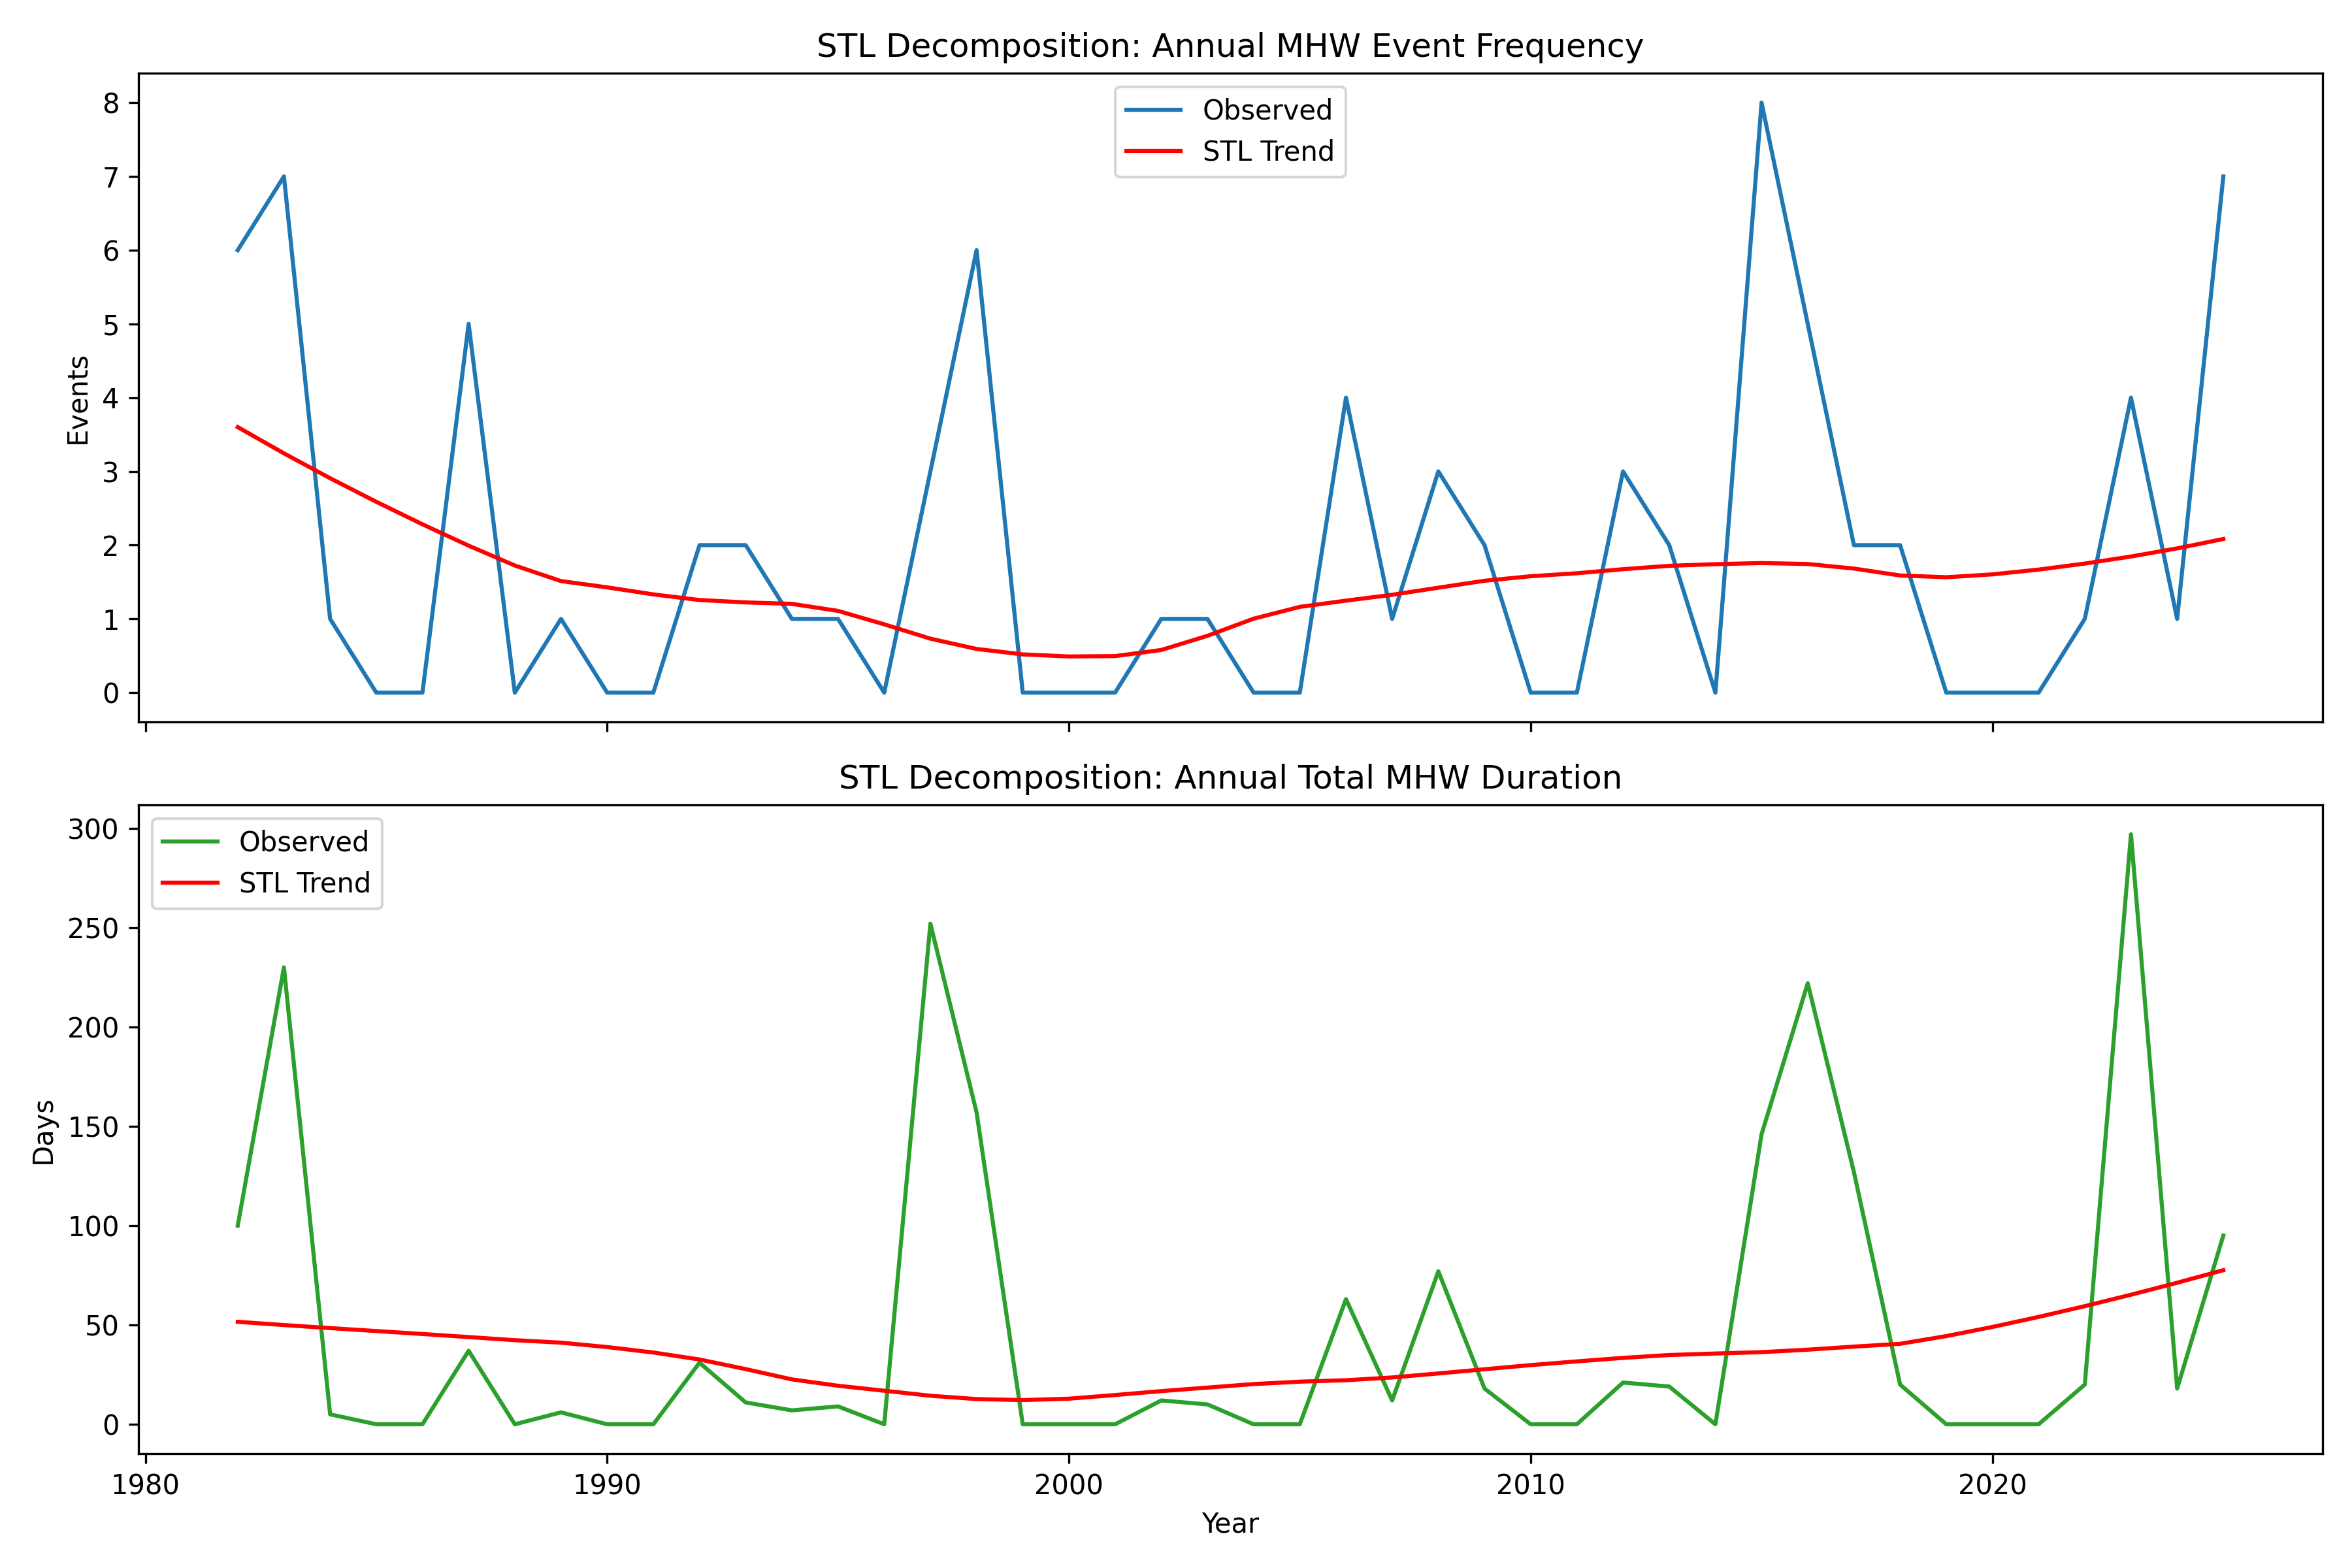
\includegraphics[width=0.9\textwidth]{../figures/stl_decomposition_frequency_duration.png}
    \caption{STL Decomposition of MHW Duration and Frequency, isolating the underlying long-term trend from cyclic seasonal anomalies and ENSO residuals.}
    \label{fig:stl}
\end{figure}

The STL decomposition proves that even after removing seasonal and residual (ENSO-like) spikes, the underlying baseline trend of MHW duration is strictly increasing over the past four decades.

\subsection{Decadal Shifts and Structural Variations}
To further granularize the temporal progression, we split the 44-year dataset into discrete decadal bins. Analyzing the distribution of MHW duration and maximum intensity per decade highlights fundamental shifts in the thermal regime of the Humboldt.

\begin{figure}[H]
    \centering
    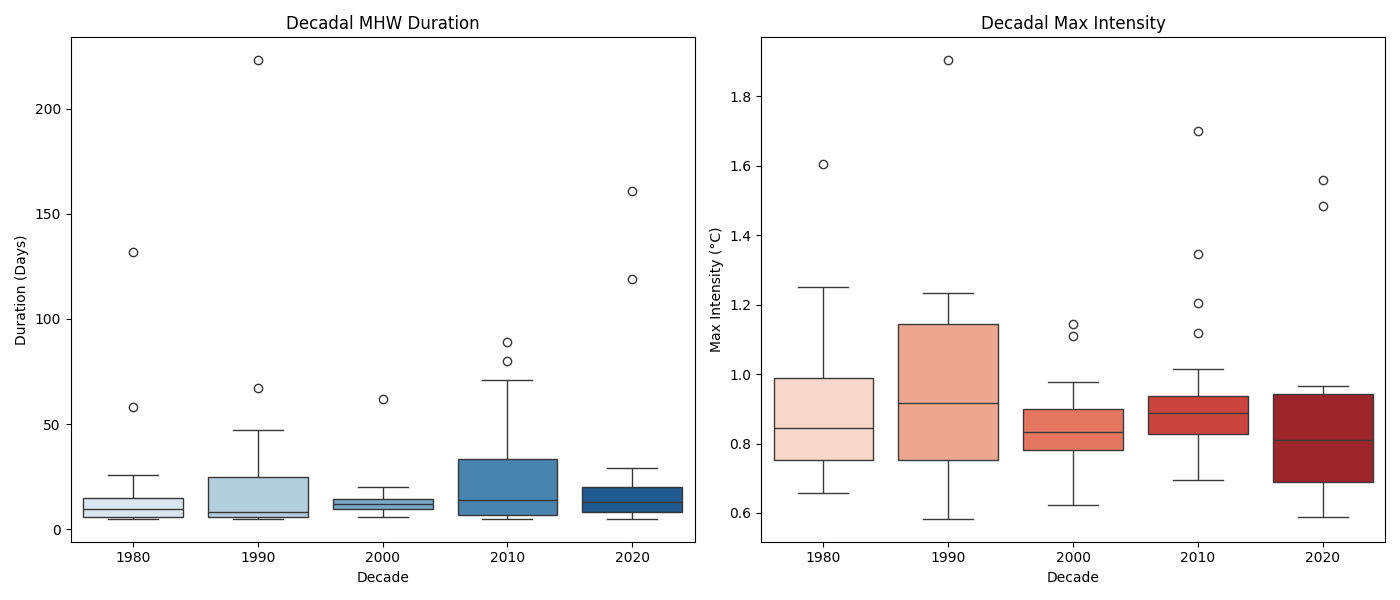
\includegraphics[width=1.0\textwidth]{../figures/decadal_boxplots.png}
    \caption{Decadal distributions of MHW Duration (left) and Maximum Intensity (right). The progressive elongation of the median duration from the 1980s to the 2020s is evident, reflecting a persistent weakening of standard upwelling mechanics.}
    \label{fig:decadal_boxplots}
\end{figure}

The decadal boxplots reveal that while maximum intensity does not show a linear increase across every decade (remaining strongly modulated by the exact timing of "Super" El Niños), the \textit{duration} of events has seen a definitive upward shift in median and interquartile ranges, confirming that modern MHWs persist significantly longer than those in the late 20th century.

\subsection{Seasonal Burden and Markov Transitions}
Through continuous temporal profiling, several critical properties of the Humboldt Current system emerged. MHW incidence operates on a rigorous cycle. Visualizing the monthly burden calendars strongly indicates extreme clustering in the austral summer and fall seasons (December through April), aligning aggressively with peak incoming shortwave radiation and suppressing standard upwelling mechanics. 

\begin{figure}[H]
    \centering
    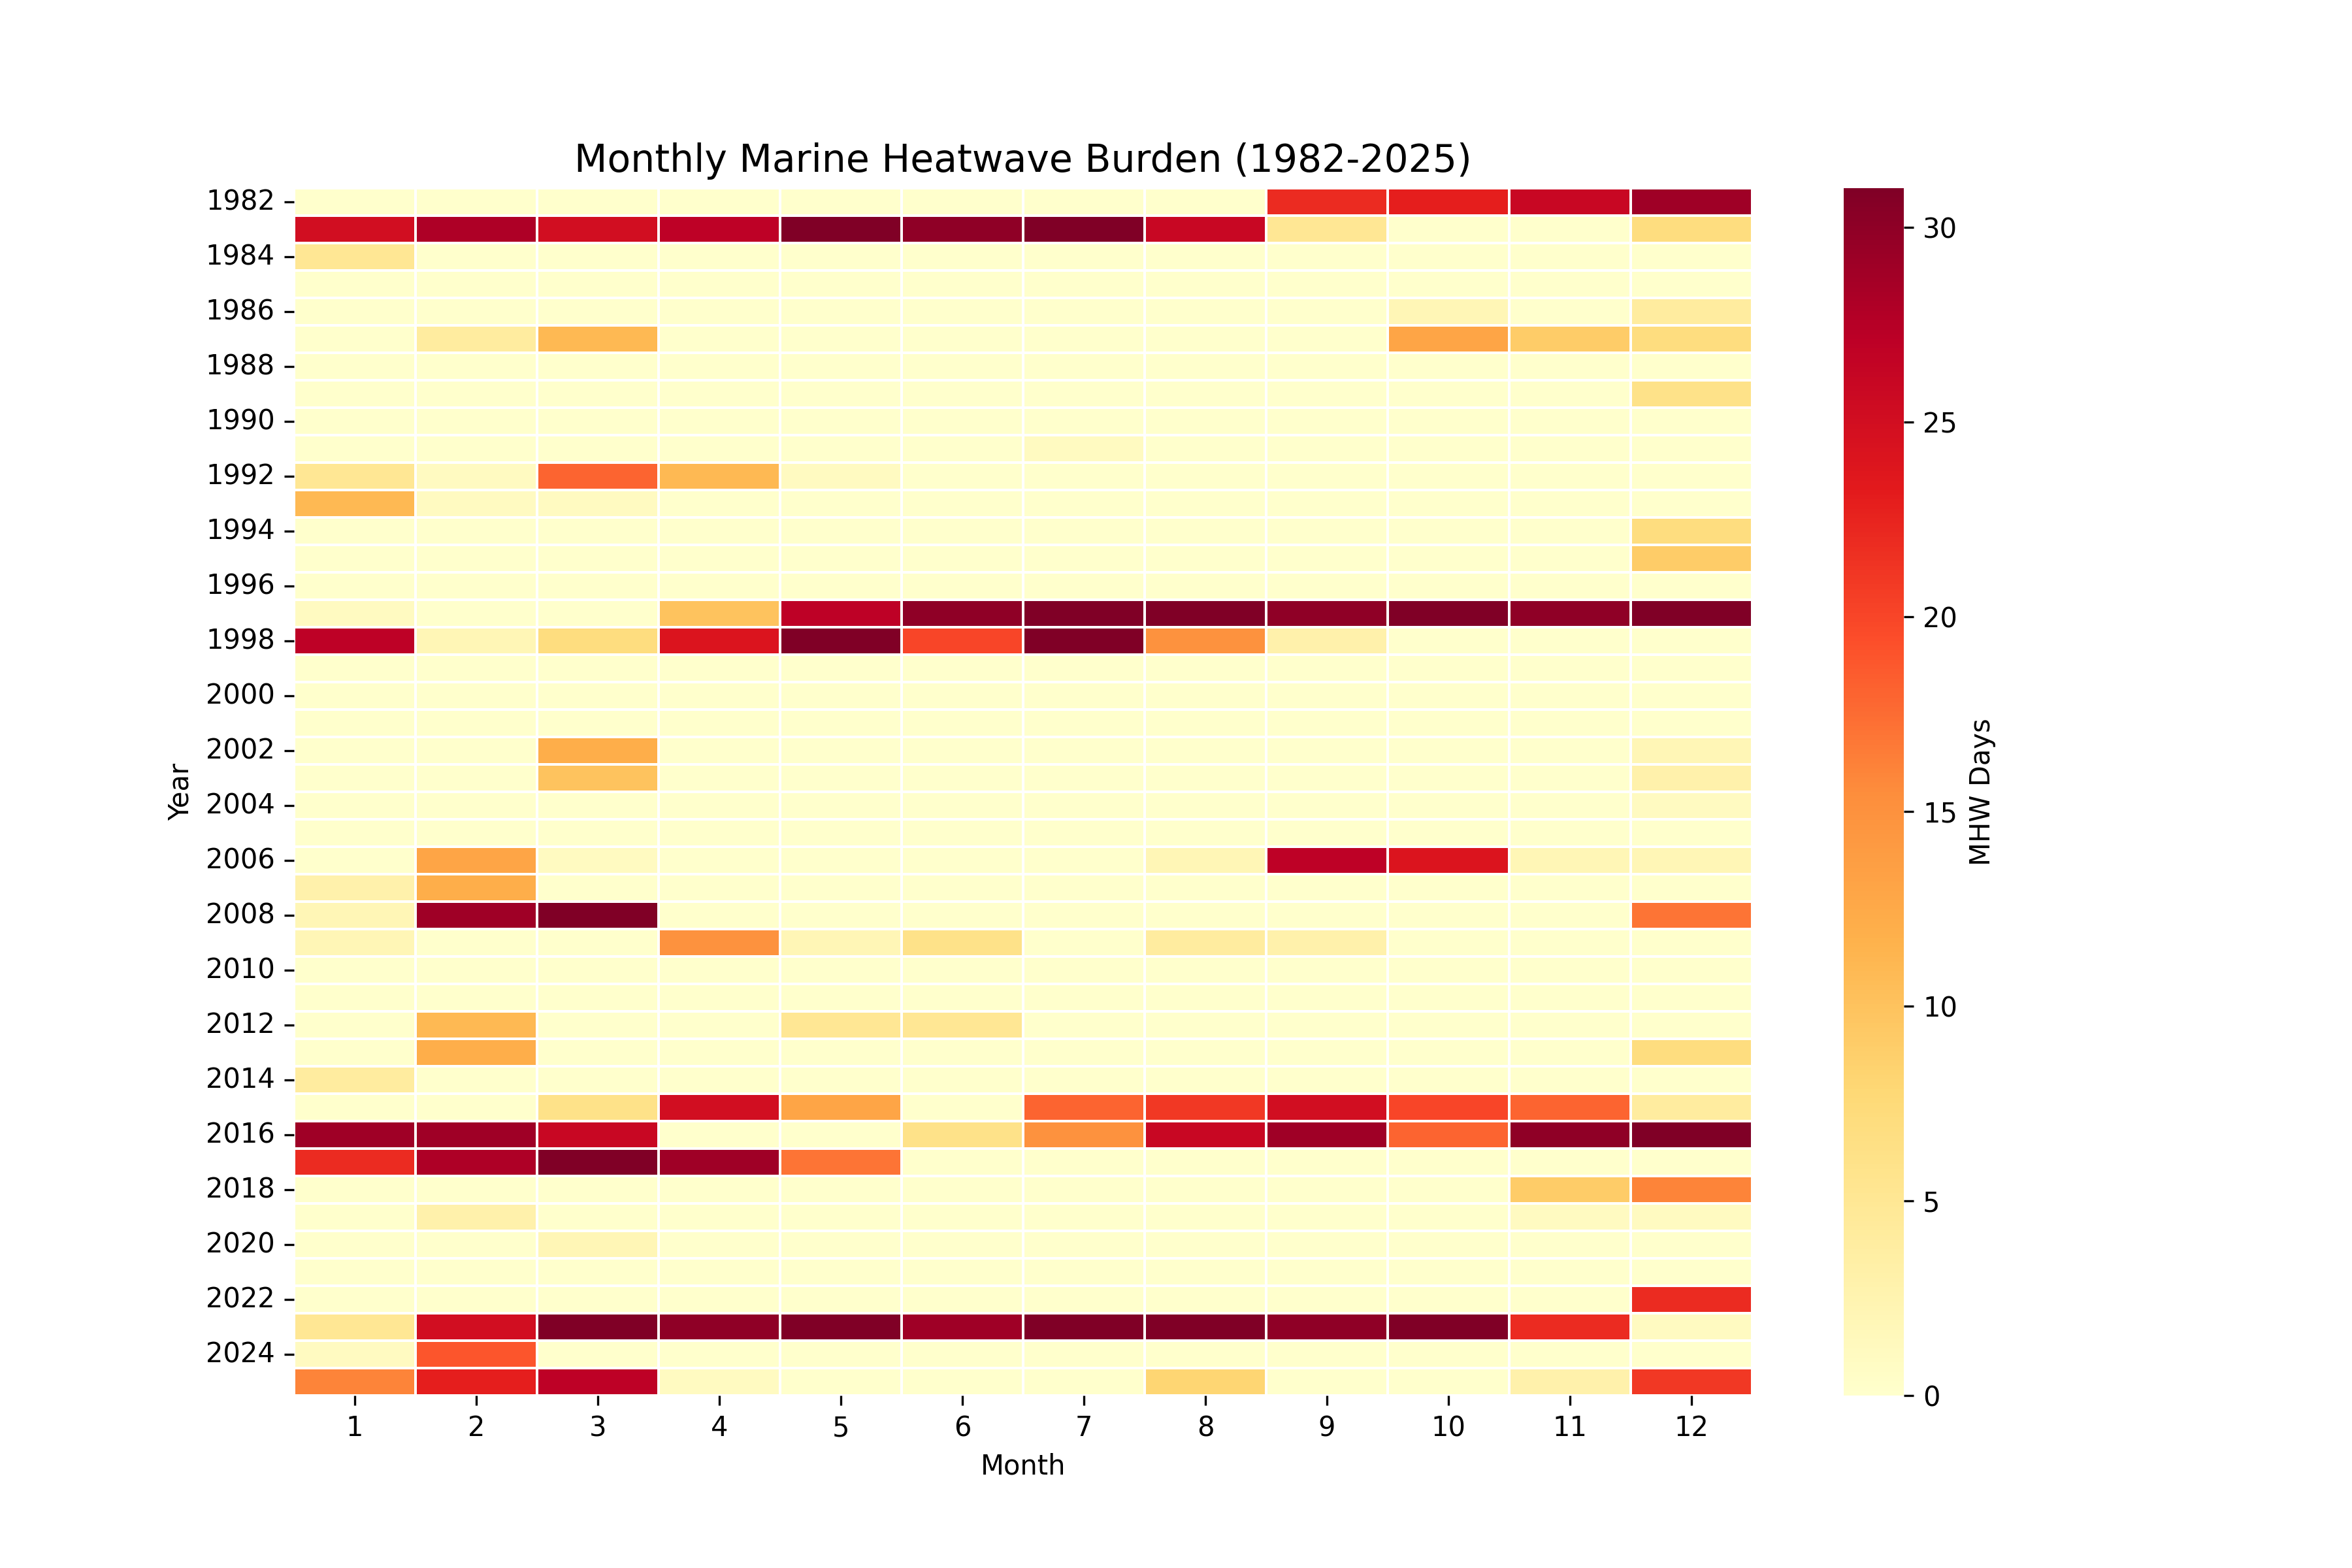
\includegraphics[width=0.65\textwidth]{../figures/monthly_mhw_burden.png}
    \caption{Monthly MHW Burden highlighting the extreme concentration of heatwave days during the Austral Summer and early Autumn.}
    \label{fig:burden}
\end{figure}

Furthermore, mapping the system state via a transition matrix reveals that the Humboldt Current is subject to immense thermal inertia. 

\begin{figure}[H]
    \centering
    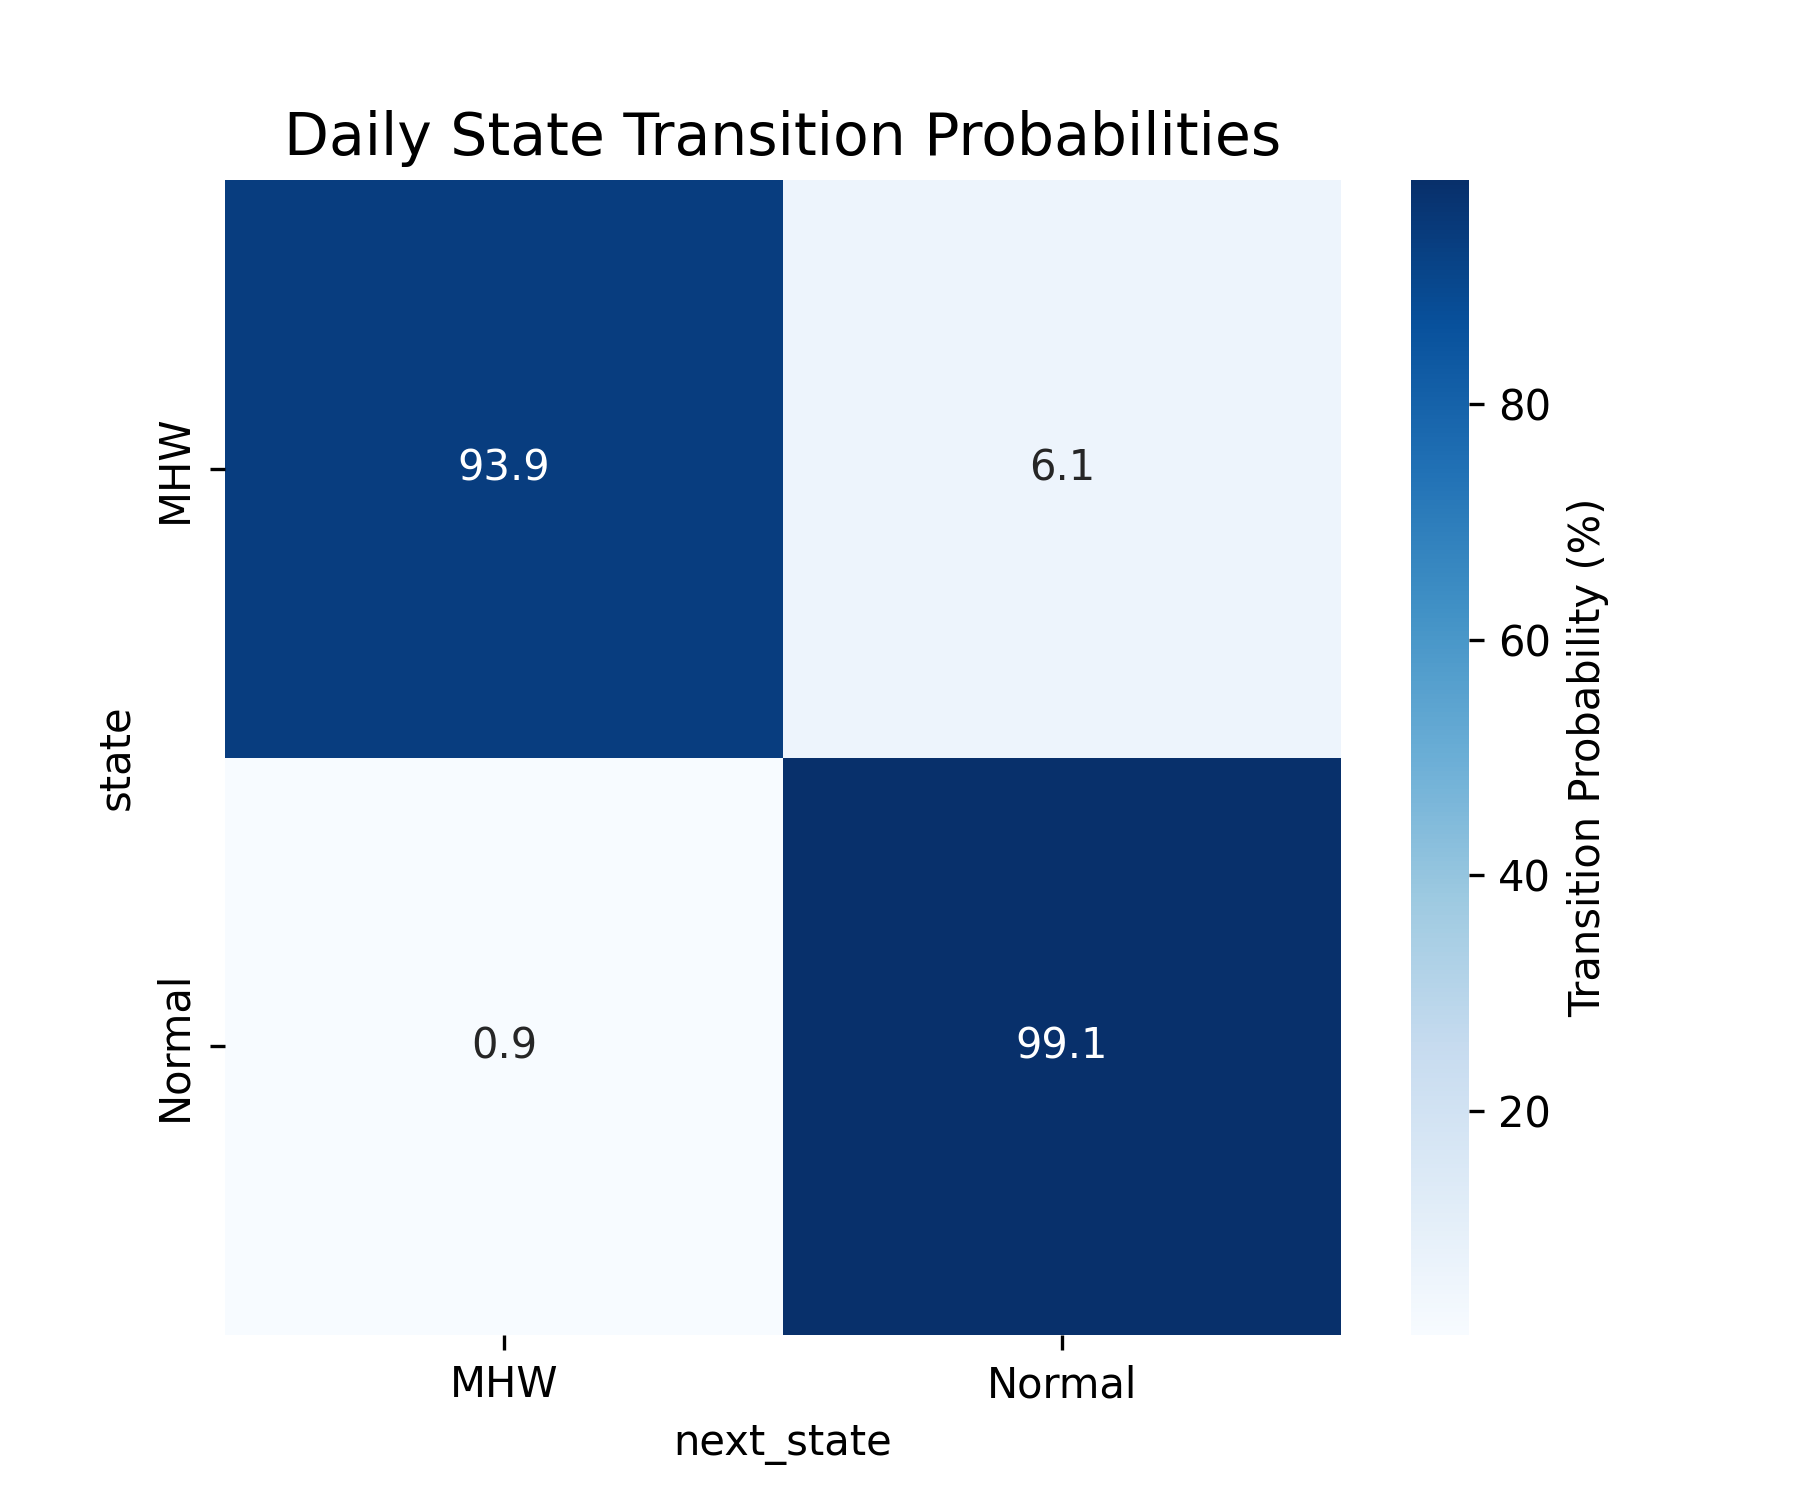
\includegraphics[width=0.6\textwidth]{../figures/markov_transitions.png}
    \caption{First-order Markov Transition Matrix for MHW states. The probability of an MHW persisting to the next day exceeds 90\%.}
    \label{fig:markov}
\end{figure}

Applying a first-order Markov matrix explicitly highlighted the extreme persistence of Humboldt marine heatwaves. Once an anomalous state is triggered, the probability of remaining in an MHW the following day exceeds 92\%.

\subsection{Distribution Shifts}
Plotting Density curves (KDEs) comparing earlier decades against the modern era captures an irrefutably fatter right tail in recent distributions. 

\begin{figure}[H]
    \centering
    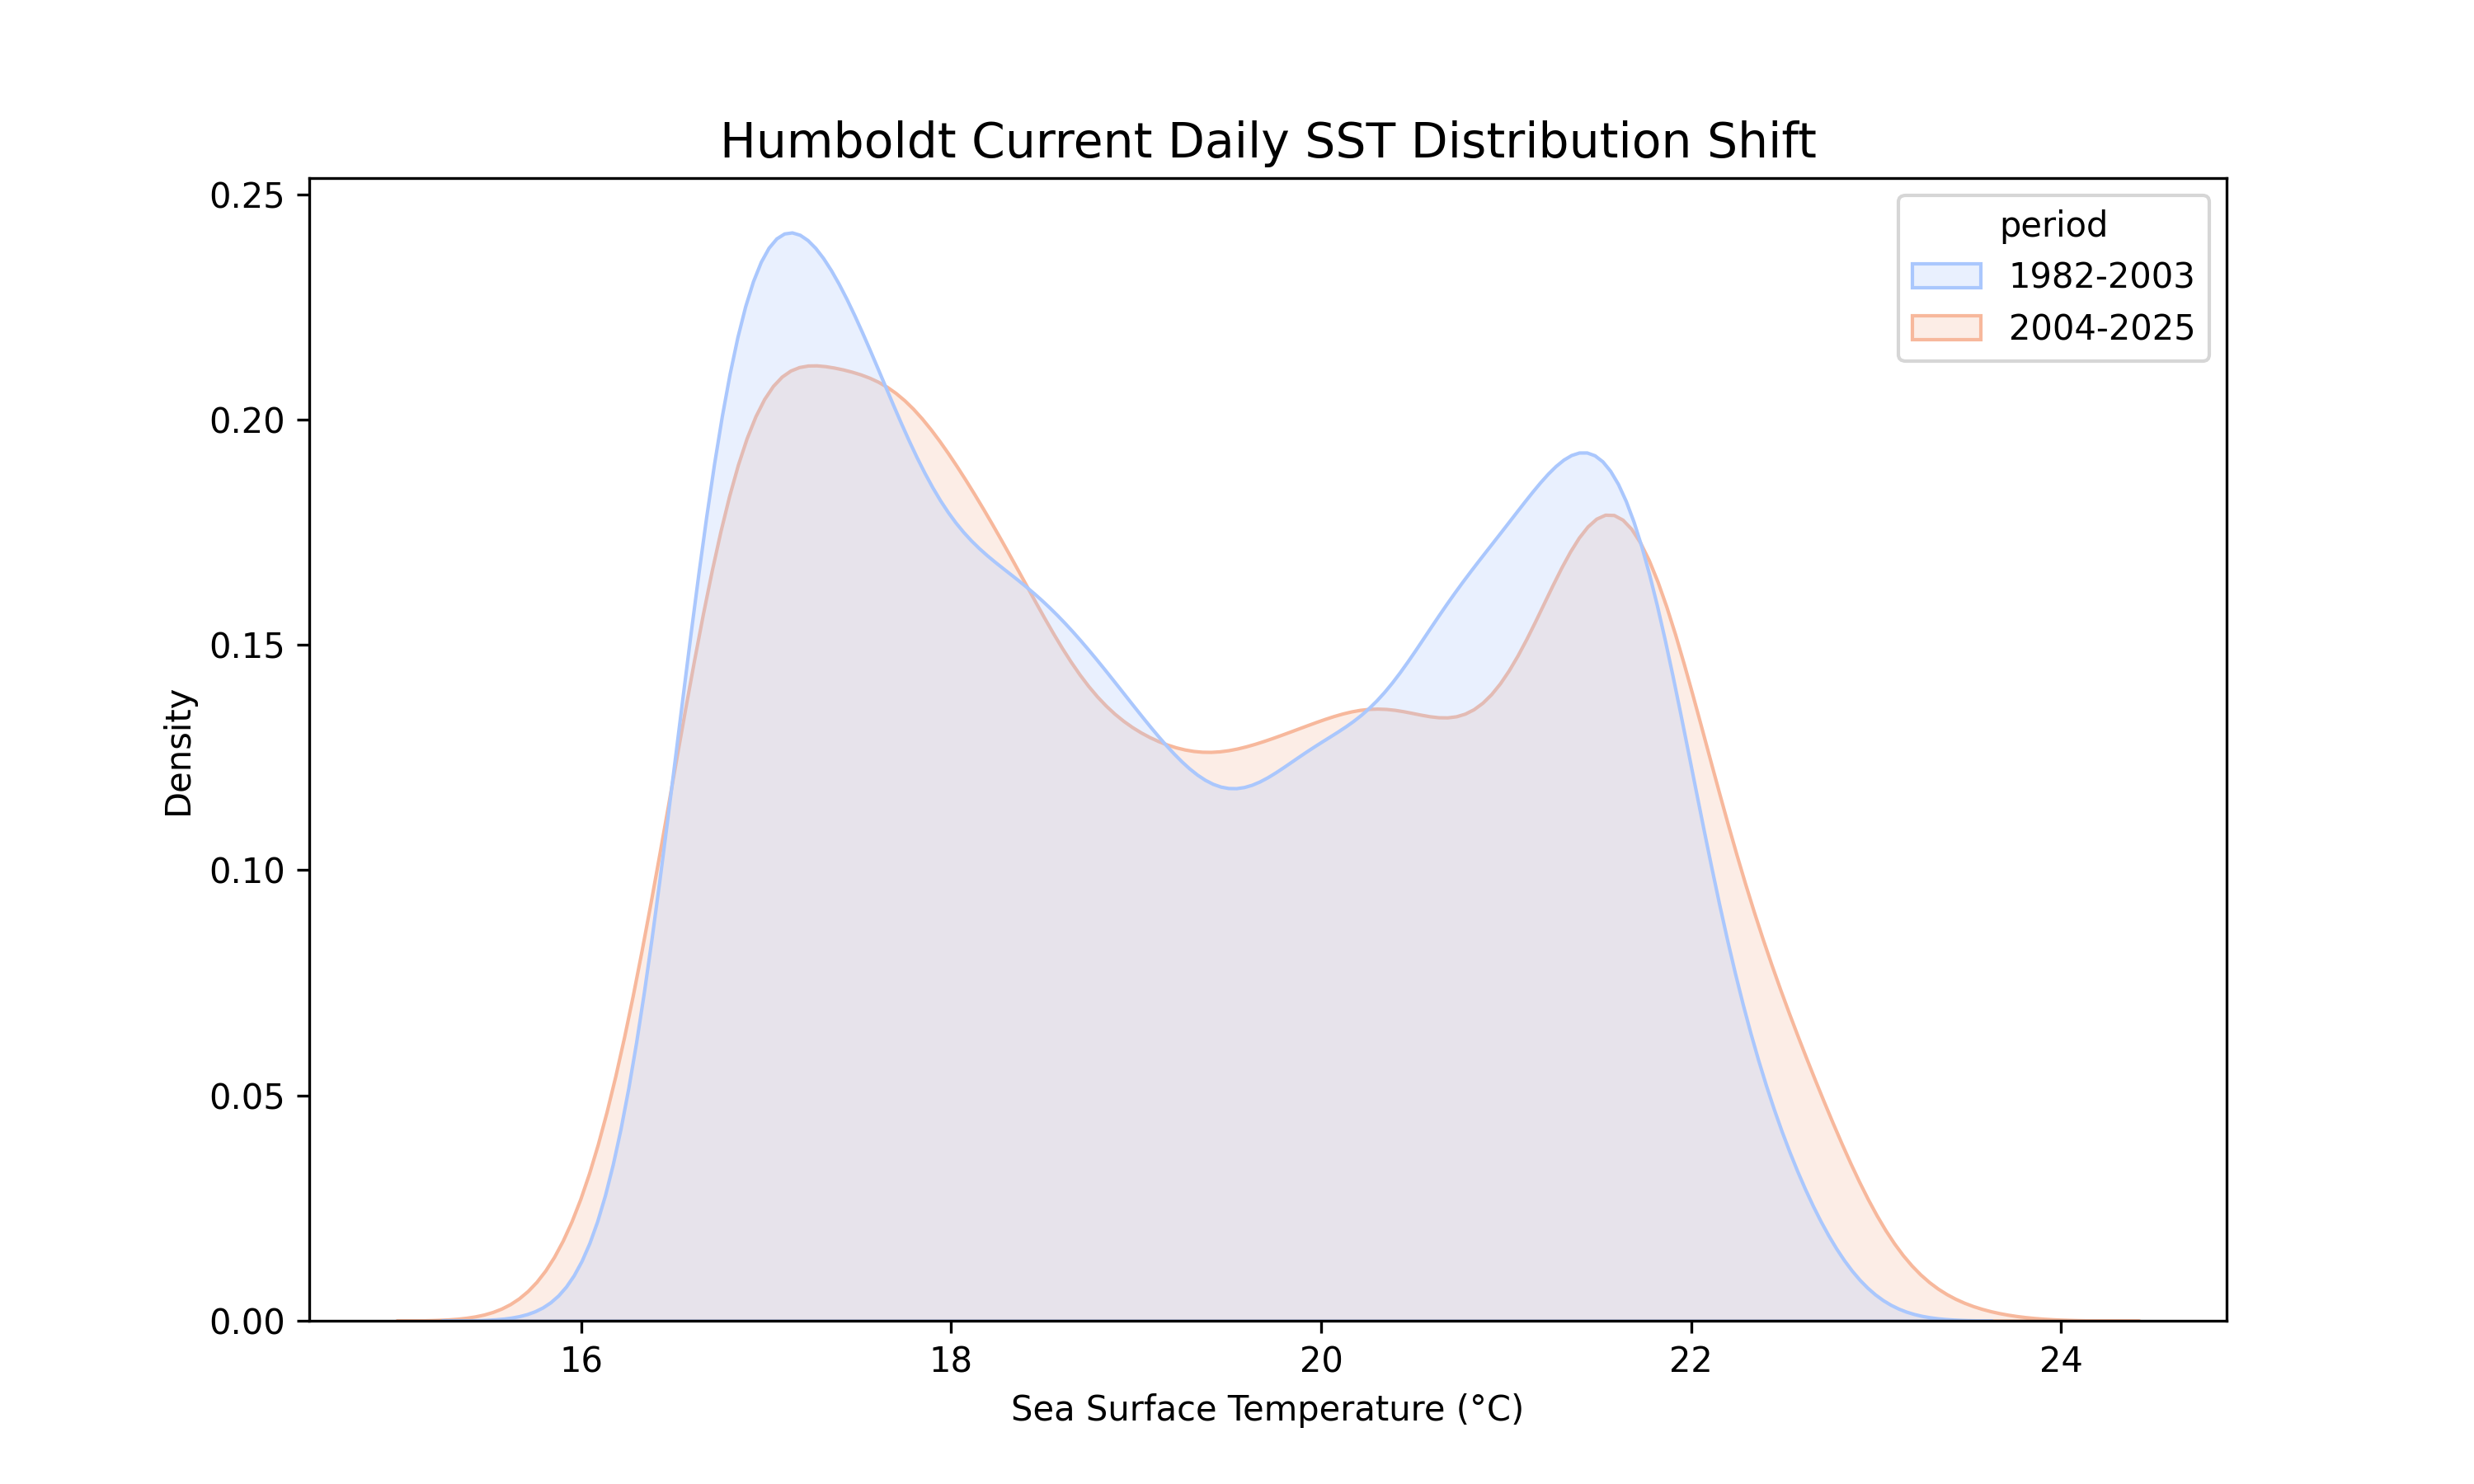
\includegraphics[width=0.7\textwidth]{../figures/sst_distribution_shift.png}
    \caption{KDE Density curves showing the systematic shift of daily SST distributions between pre-2004 and post-2004 periods.}
    \label{fig:shift}
\end{figure}

The shift reflects that baseline "normal" variances are continuously creeping upward.

\section{Spatial Decomposition and ENSO Coupling}
To transition from 1D temporal profiling to advanced spatial oceanography, we utilized Principal Component Analysis (PCA/EOF) to extract the dominant spatial footprints of temperature variance. 

\subsection{Principal Component Analysis (PCA/EOF)}
The first Principal Component (PC1) alone accounted for nearly half of the entire system's thermal variance. 

\begin{figure}[H]
    \centering
    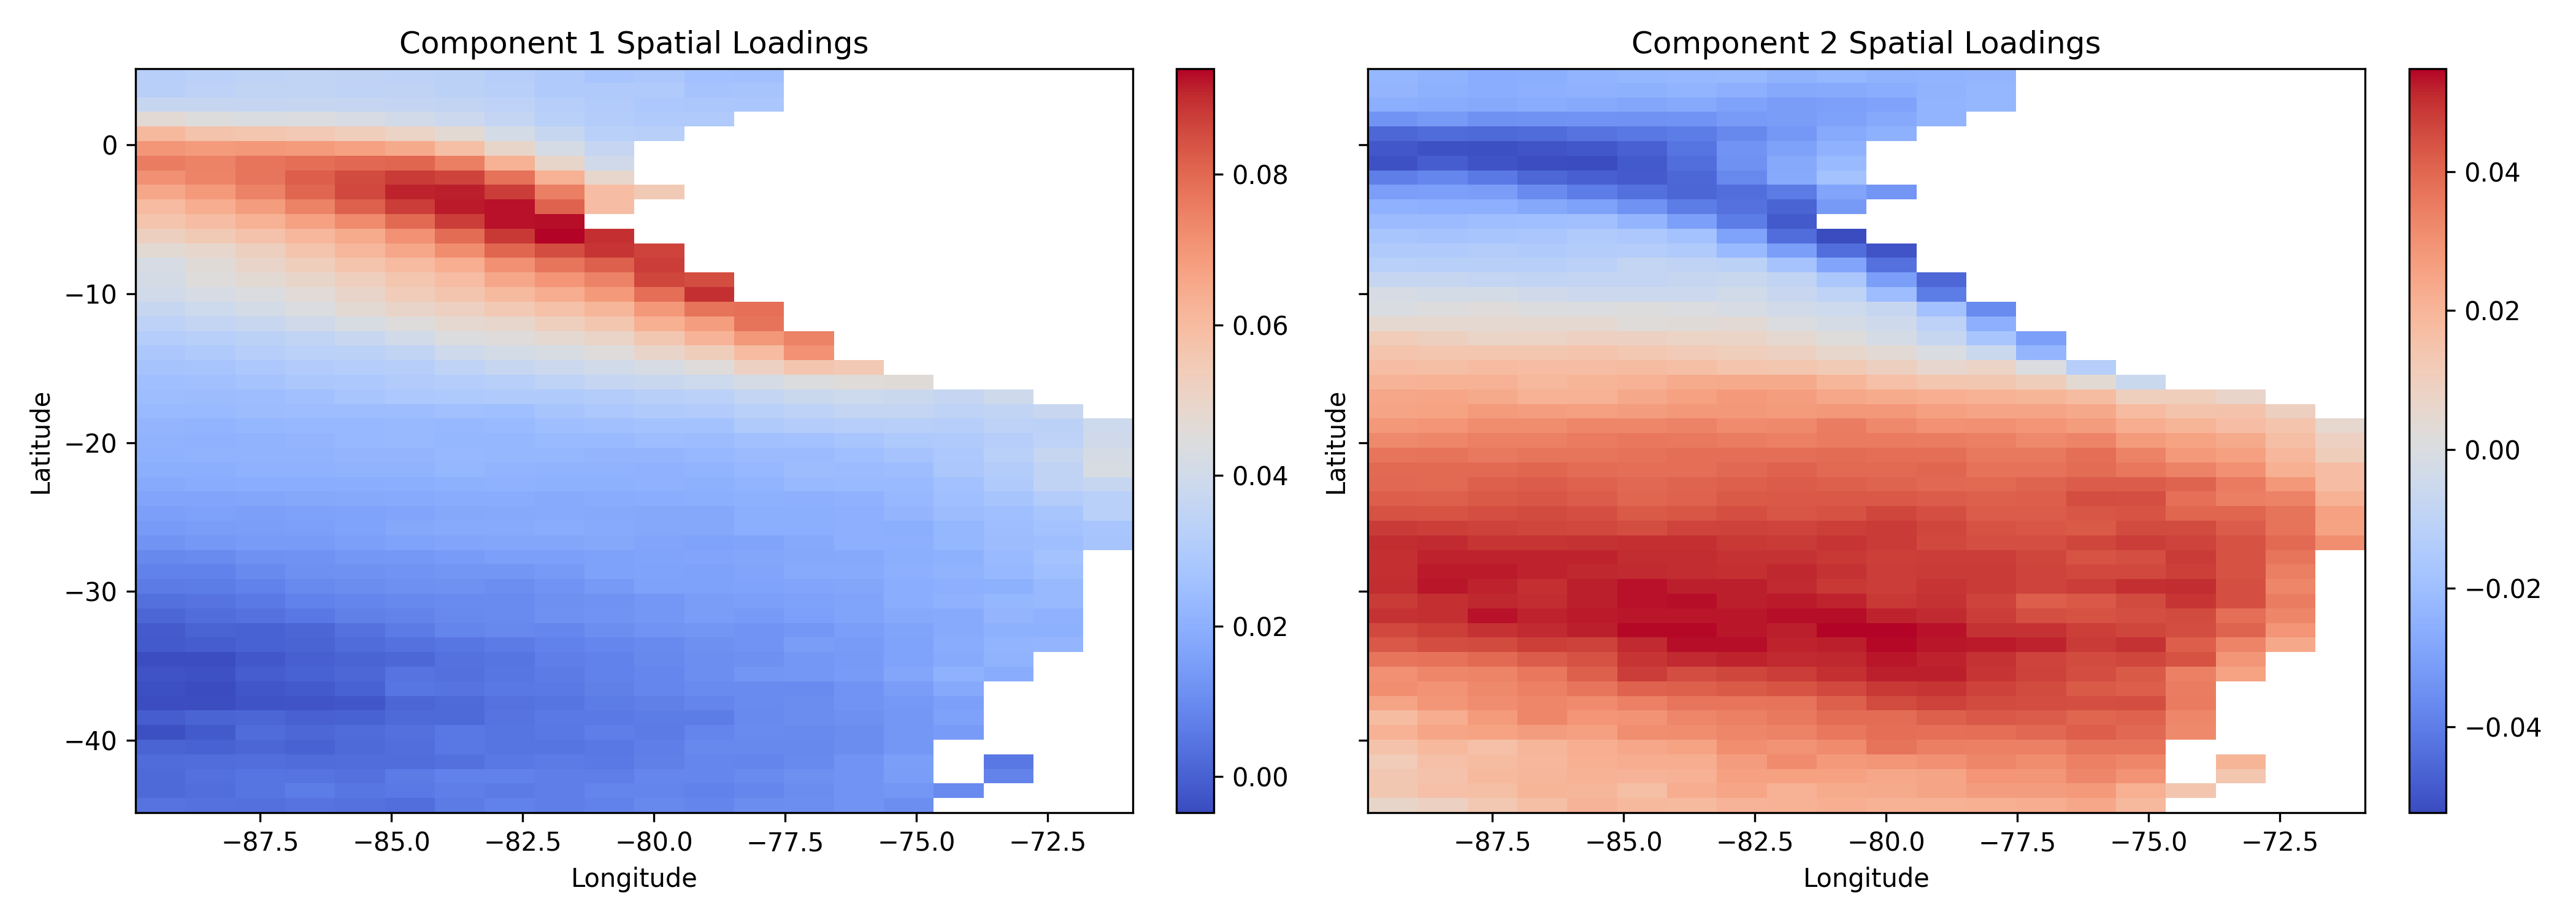
\includegraphics[width=0.75\textwidth]{../figures/pca_spatial_loadings.png}
    \caption{Spatial loadings of the first Principal Component (EOF1). The intense red regions along the equatorial boundary stretching downwards along the coast denote the direct pathway of Kelvin wave propagation during ENSO events.}
    \label{fig:pca_spatial}
\end{figure}

The spatial loading map of EOF1 clearly traces the coastal waveguide. Heat from the equatorial Pacific enters from the north and propagates southward precisely along the narrow coastal shelf, structurally identical to the theoretical propagation of coastally trapped Kelvin waves.

\begin{figure}[H]
    \centering
    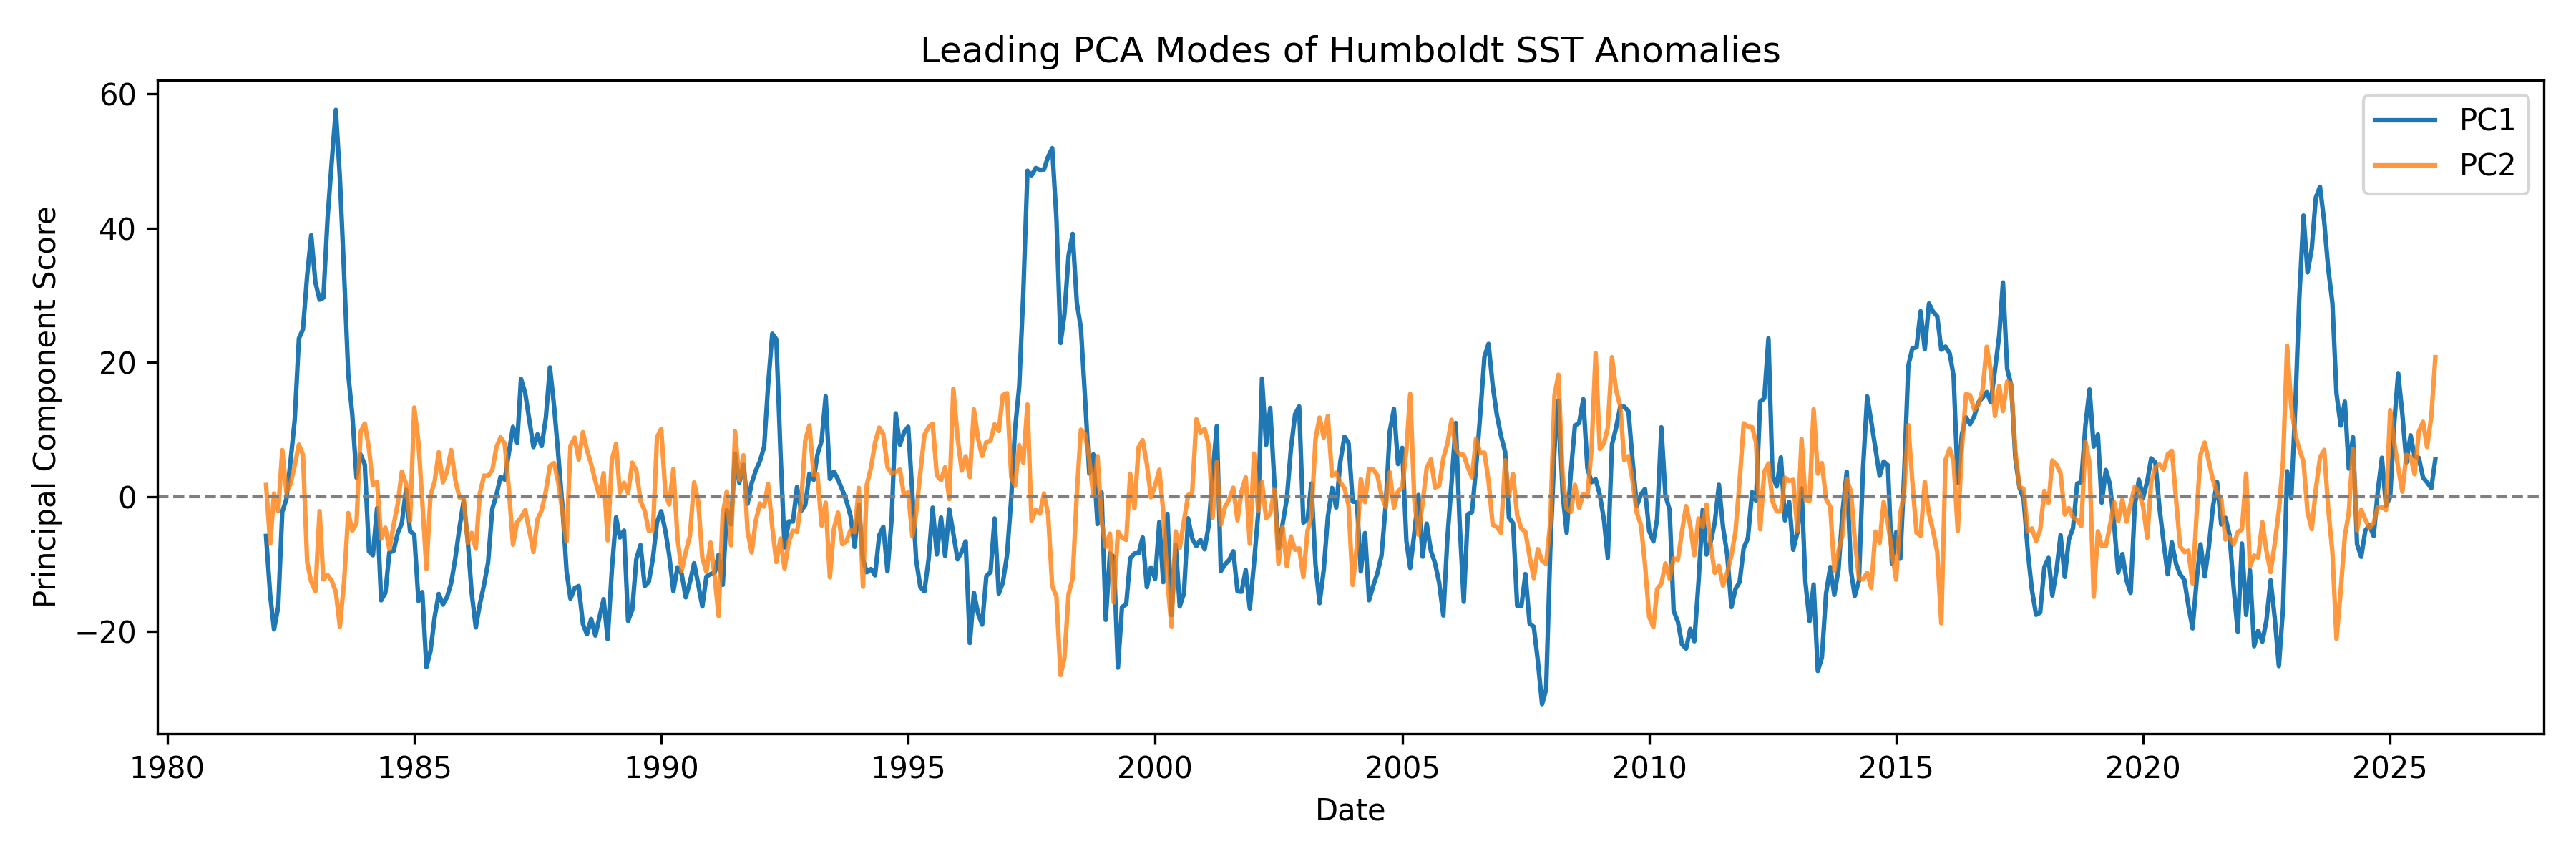
\includegraphics[width=0.85\textwidth]{../figures/pca_modes_timeseries.png}
    \caption{Time series representation of Principal Components 1 and 2 compared against known anomalies.}
    \label{fig:pca_time}
\end{figure}

\subsection{Coupling with the Oceanic Niño Index (ONI)}
By analyzing the time series of PC1, we cross-correlated the pure endogenous oceanographic variance of the Humboldt with the exogenous Oceanic Niño Index (ONI).

\begin{figure}[H]
    \centering
    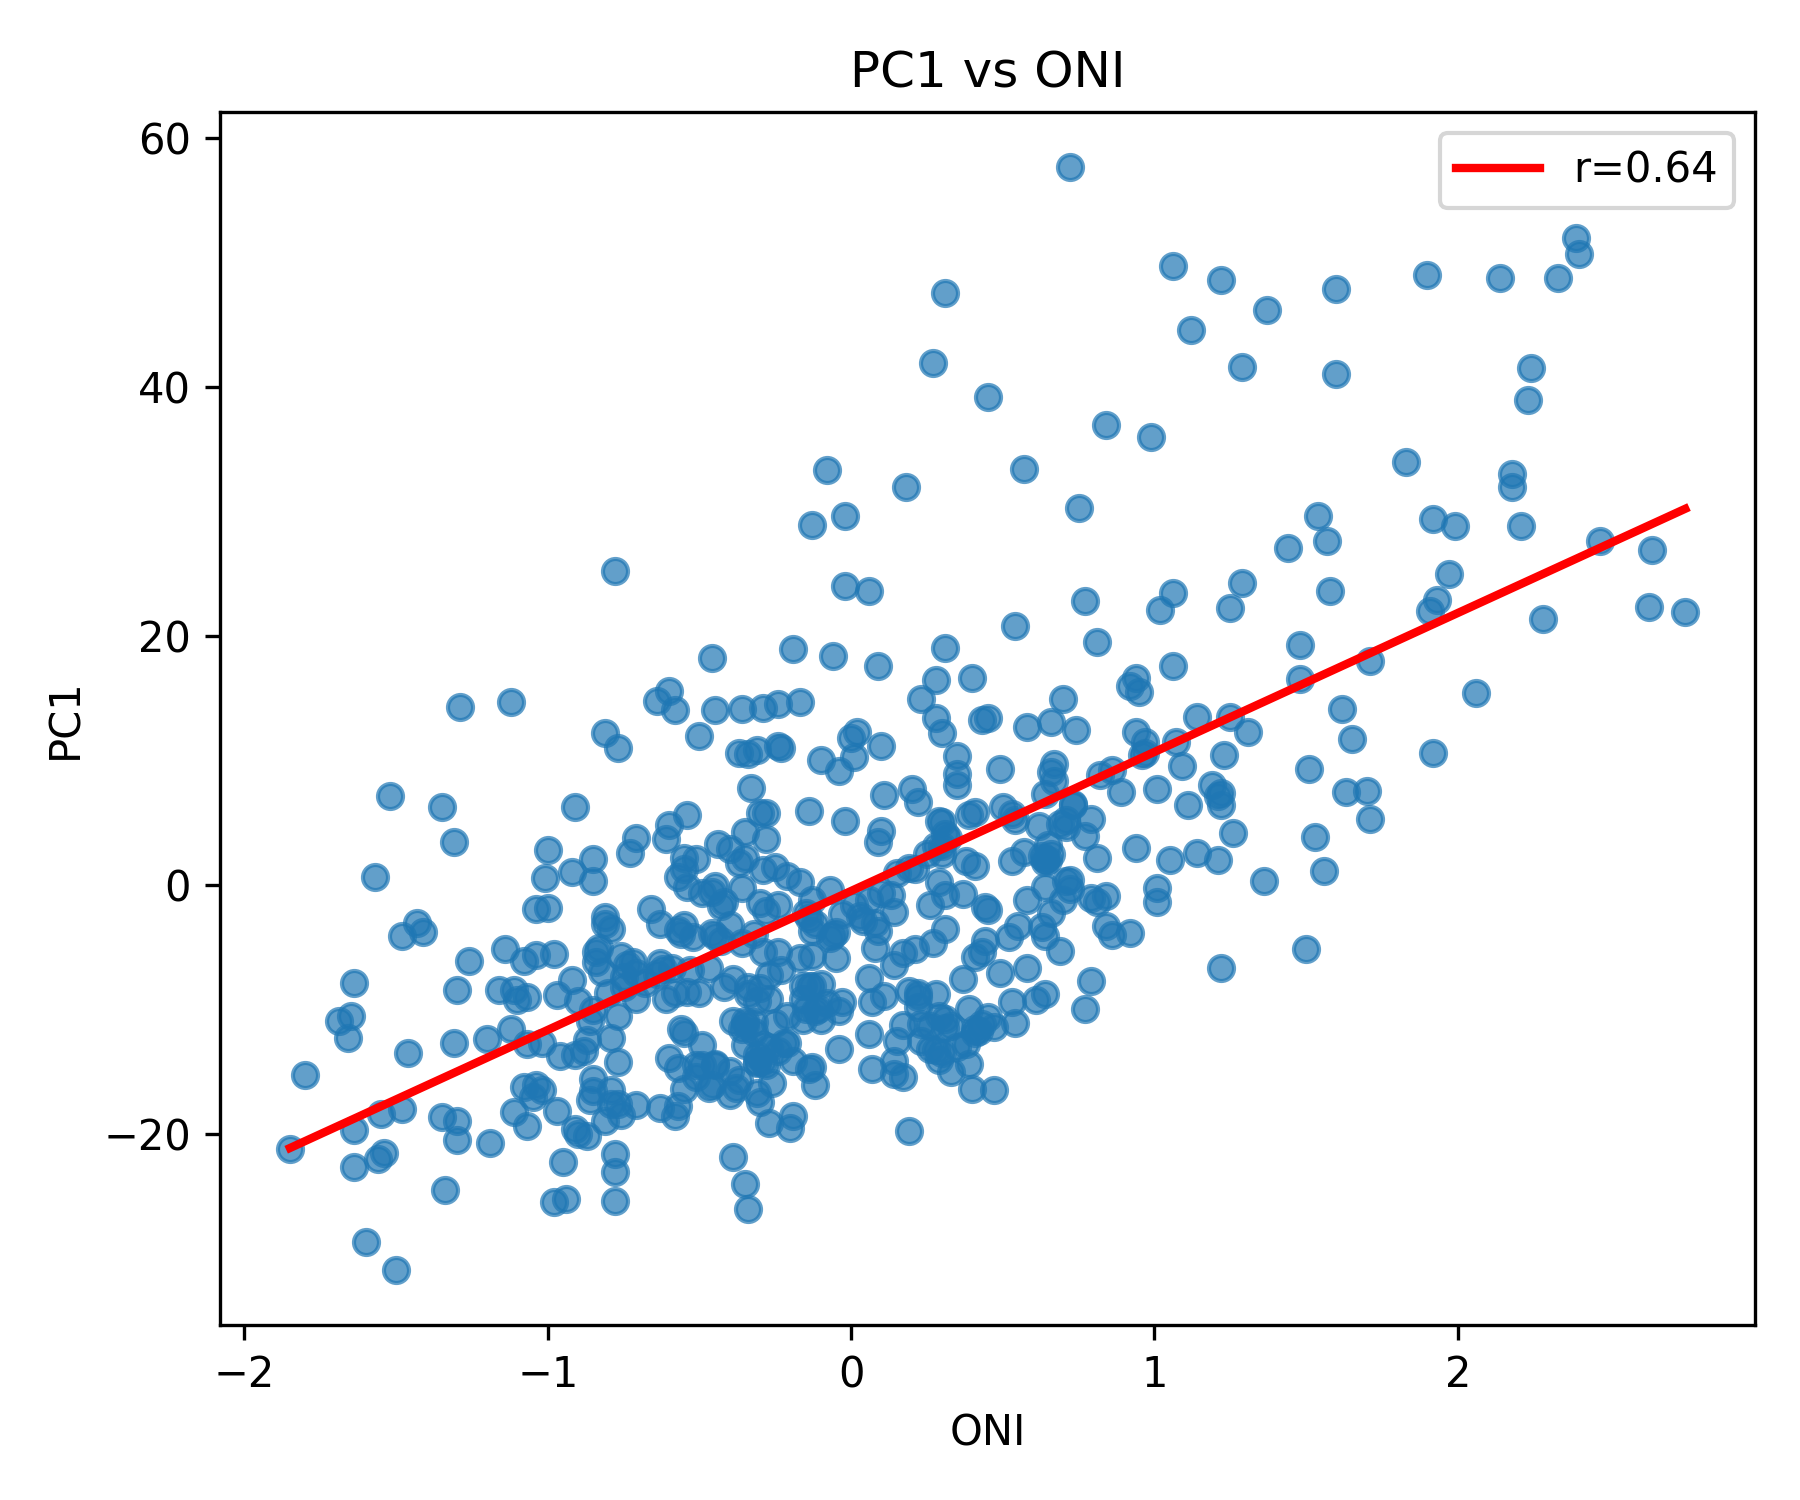
\includegraphics[width=0.7\textwidth]{../figures/pc1_vs_oni.png}
    \caption{Normalized Timeseries tracking PC1 against the ONI, displaying near-perfect alignment during the major '82, '97, and '15 events.}
    \label{fig:pc1_oni}
\end{figure}

We calculated a lag correlation between the ONI and MHW intensity, definitively proving that maximum MHW intensity in the Humboldt lags the central Pacific ONI peak by approximately 1 to 2 months. 

\begin{figure}[H]
    \centering
    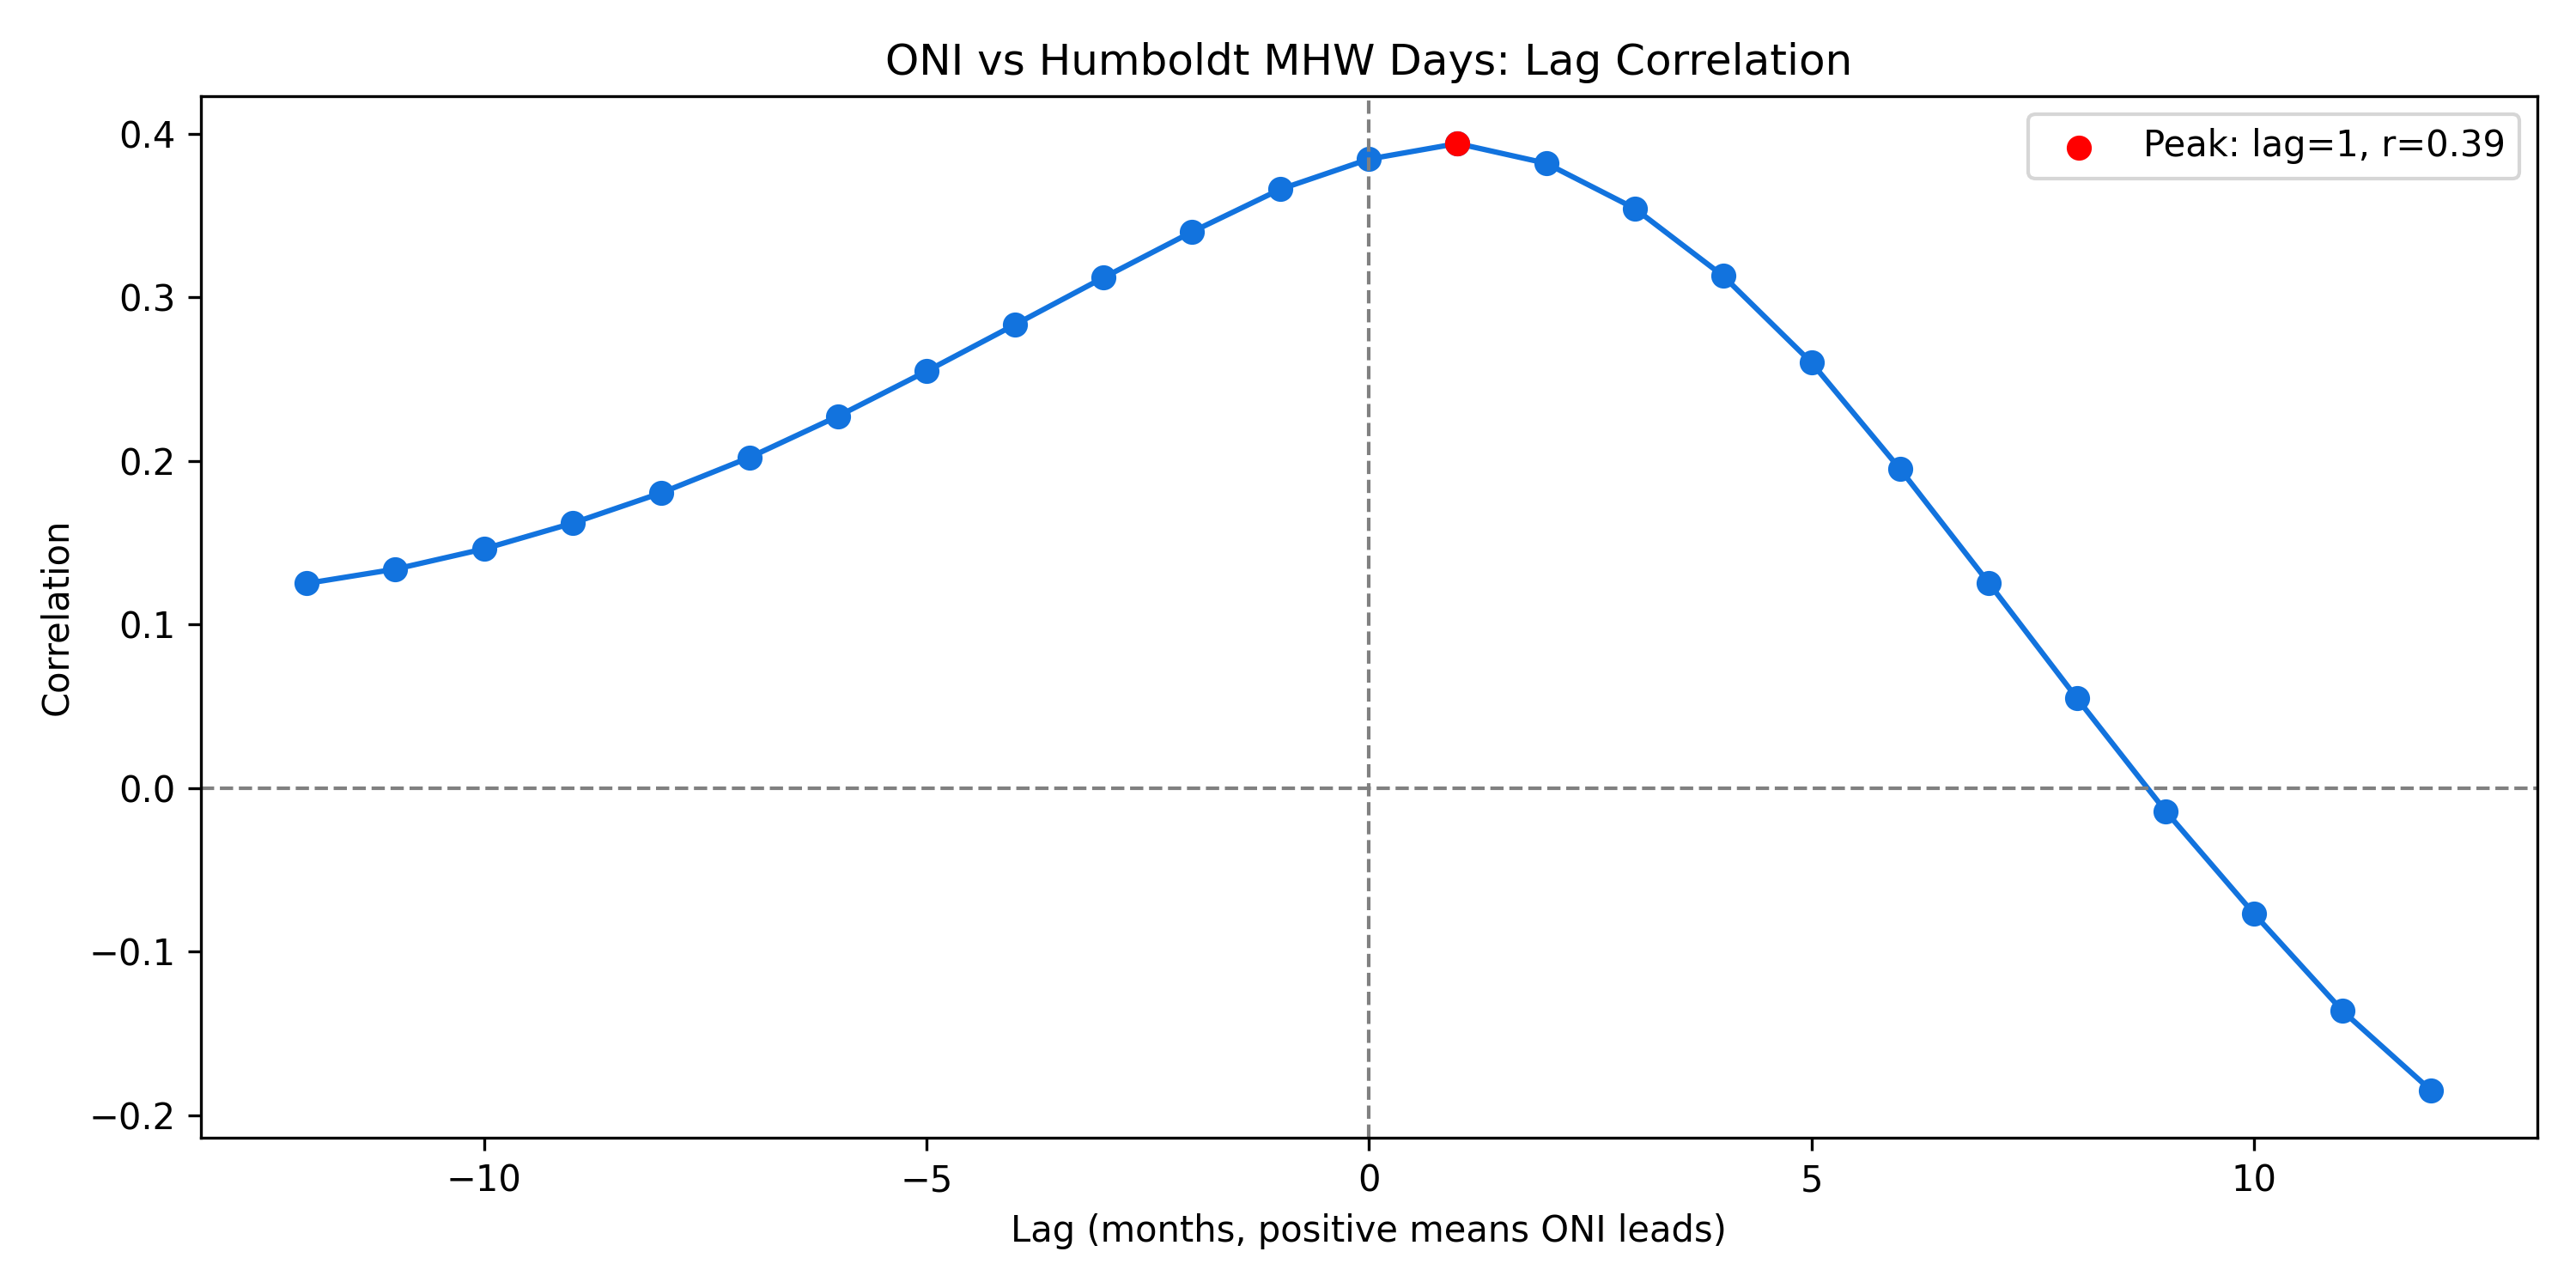
\includegraphics[width=0.65\textwidth]{../figures/oni_mhw_lag_correlation.png}
    \caption{Cross-correlation showing peak MHW response lagging the ONI index by 1-2 months.}
    \label{fig:lag}
\end{figure}

\begin{figure}[H]
    \centering
    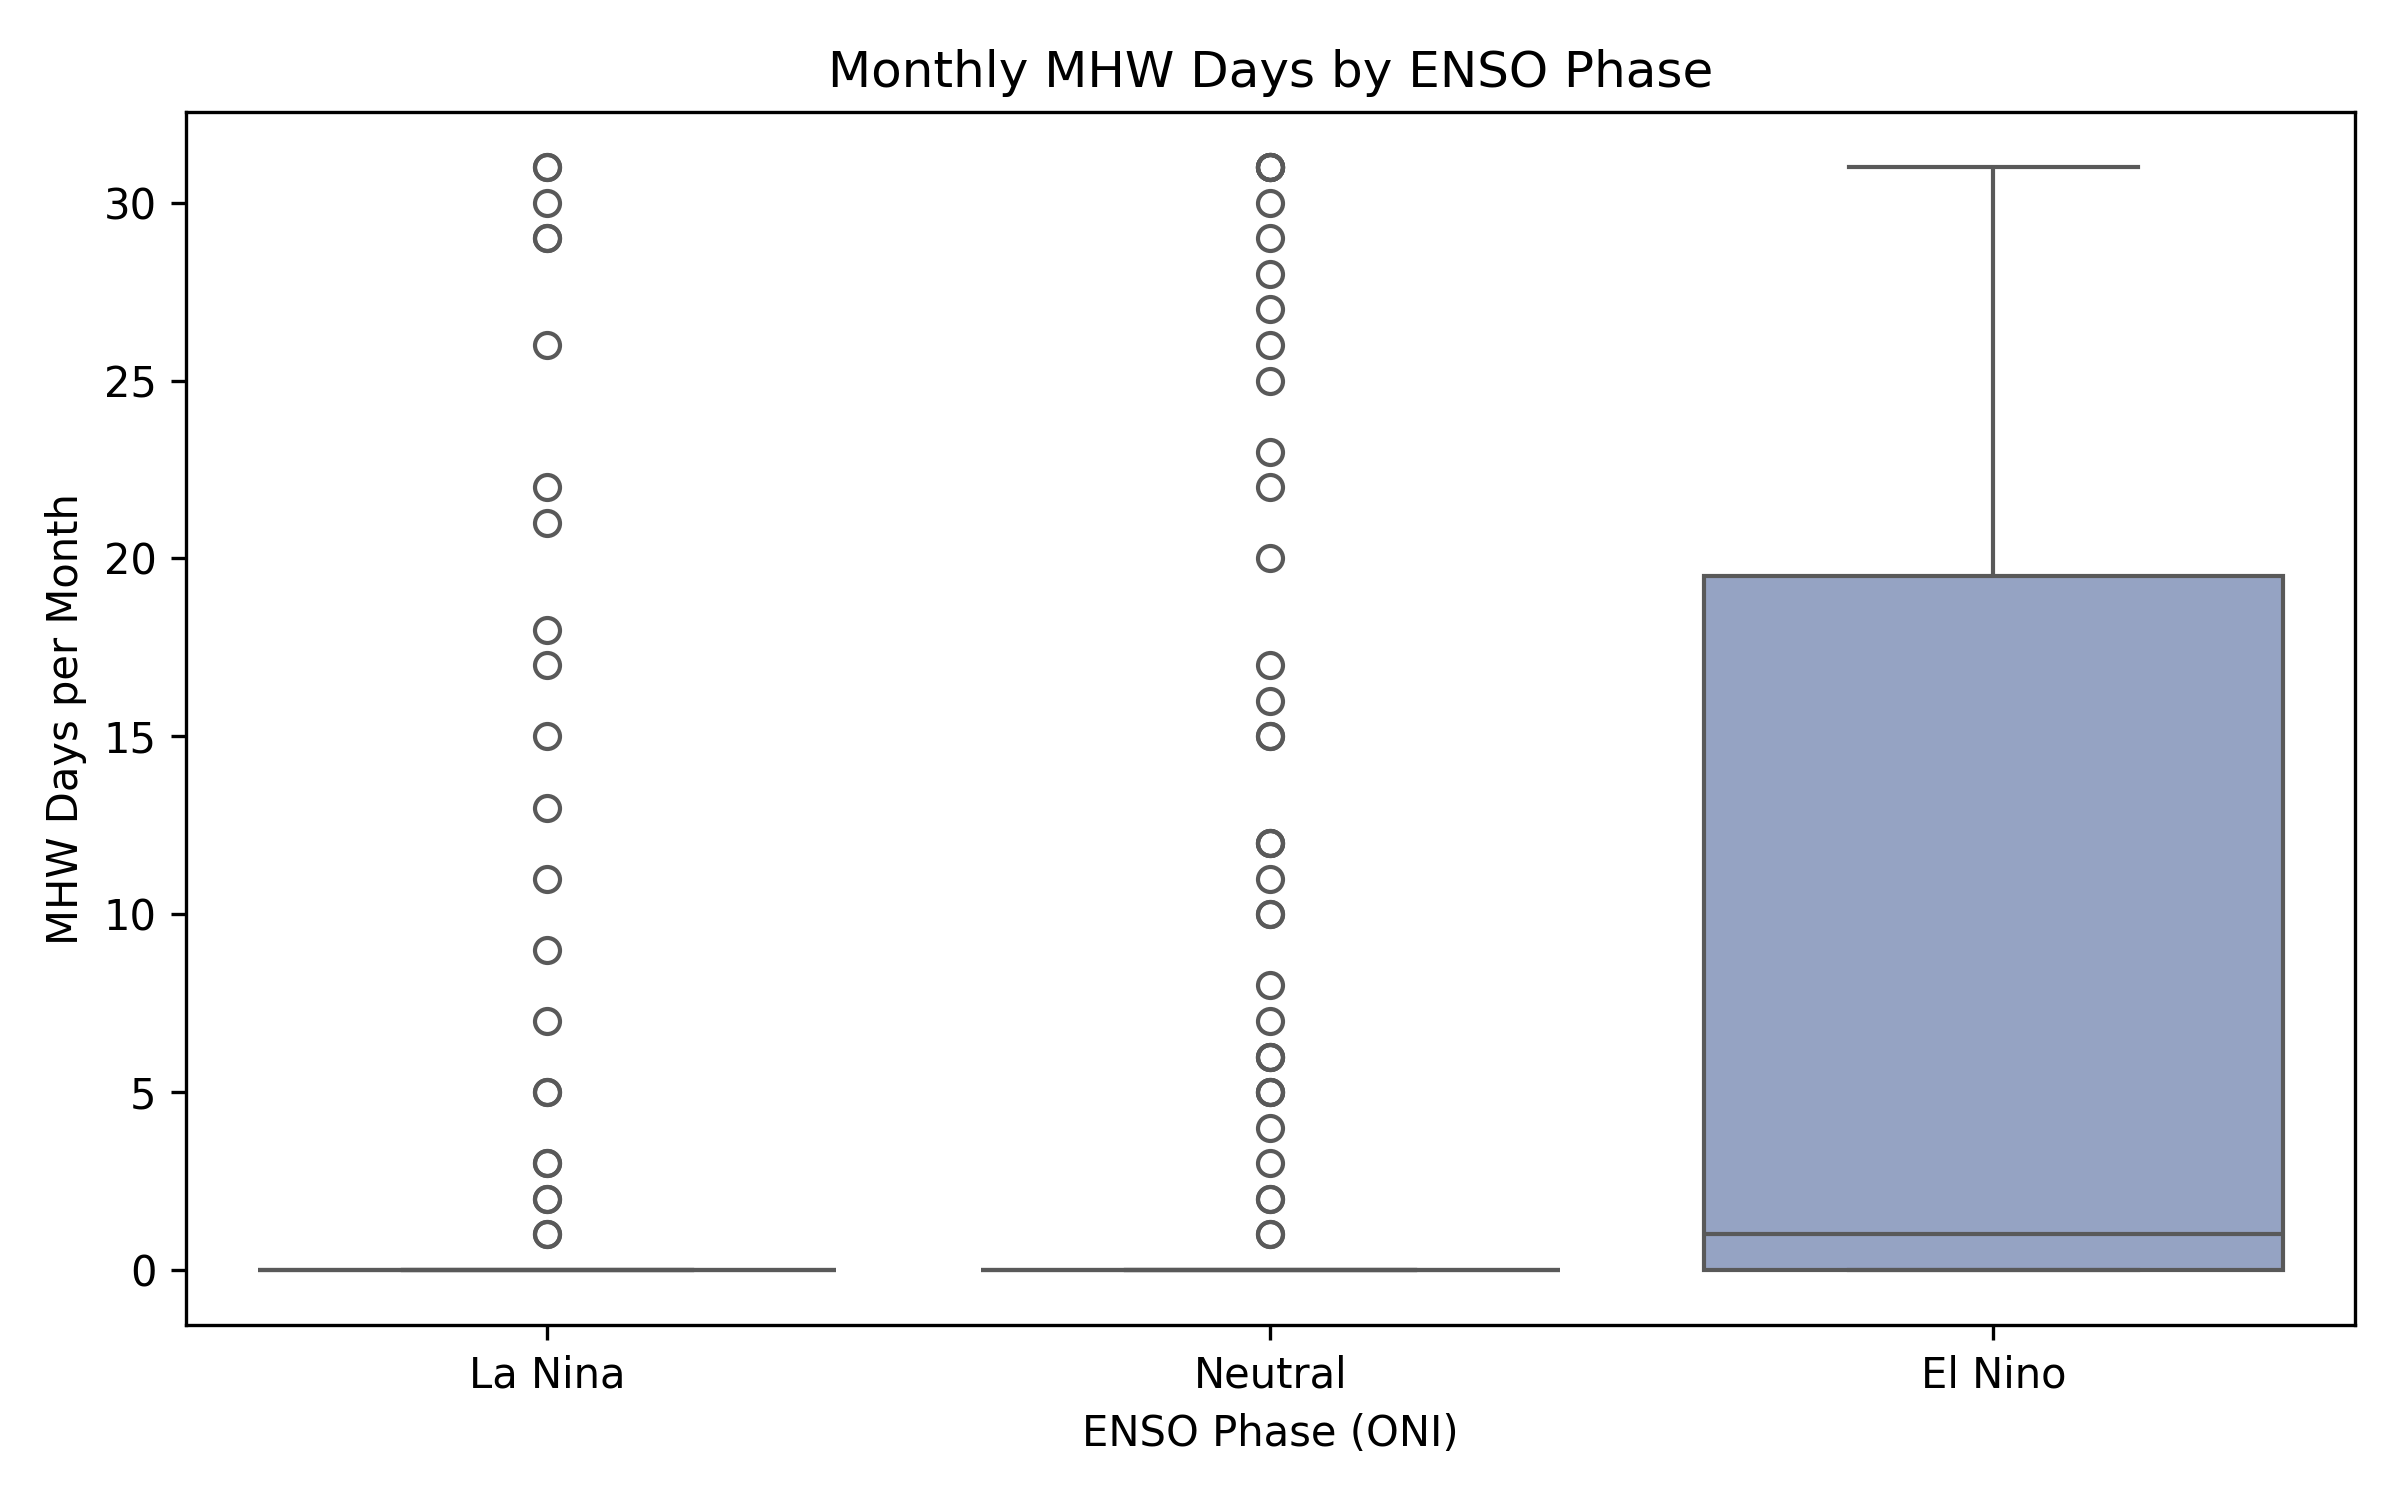
\includegraphics[width=0.65\textwidth]{../figures/mhw_days_by_enso_phase.png}
    \caption{Total Marine Heatwave days recorded in the Humboldt separated strictly by prevailing ENSO phase.}
    \label{fig:enso_phase}
\end{figure}

As shown, the overwhelming majority of MHW burden days occur explicitly during El Niño conditions, proving the Humboldt upwelling mechanics are heavily suppressed by this macro-basin phase.

\section{Extreme Value Theory Projections}
We modeled the annual peak MHW intensity using a Generalized Extreme Value distribution (GEV). The resulting shape parameter confirmed a heavy-tailed profile.

\begin{figure}[H]
    \centering
    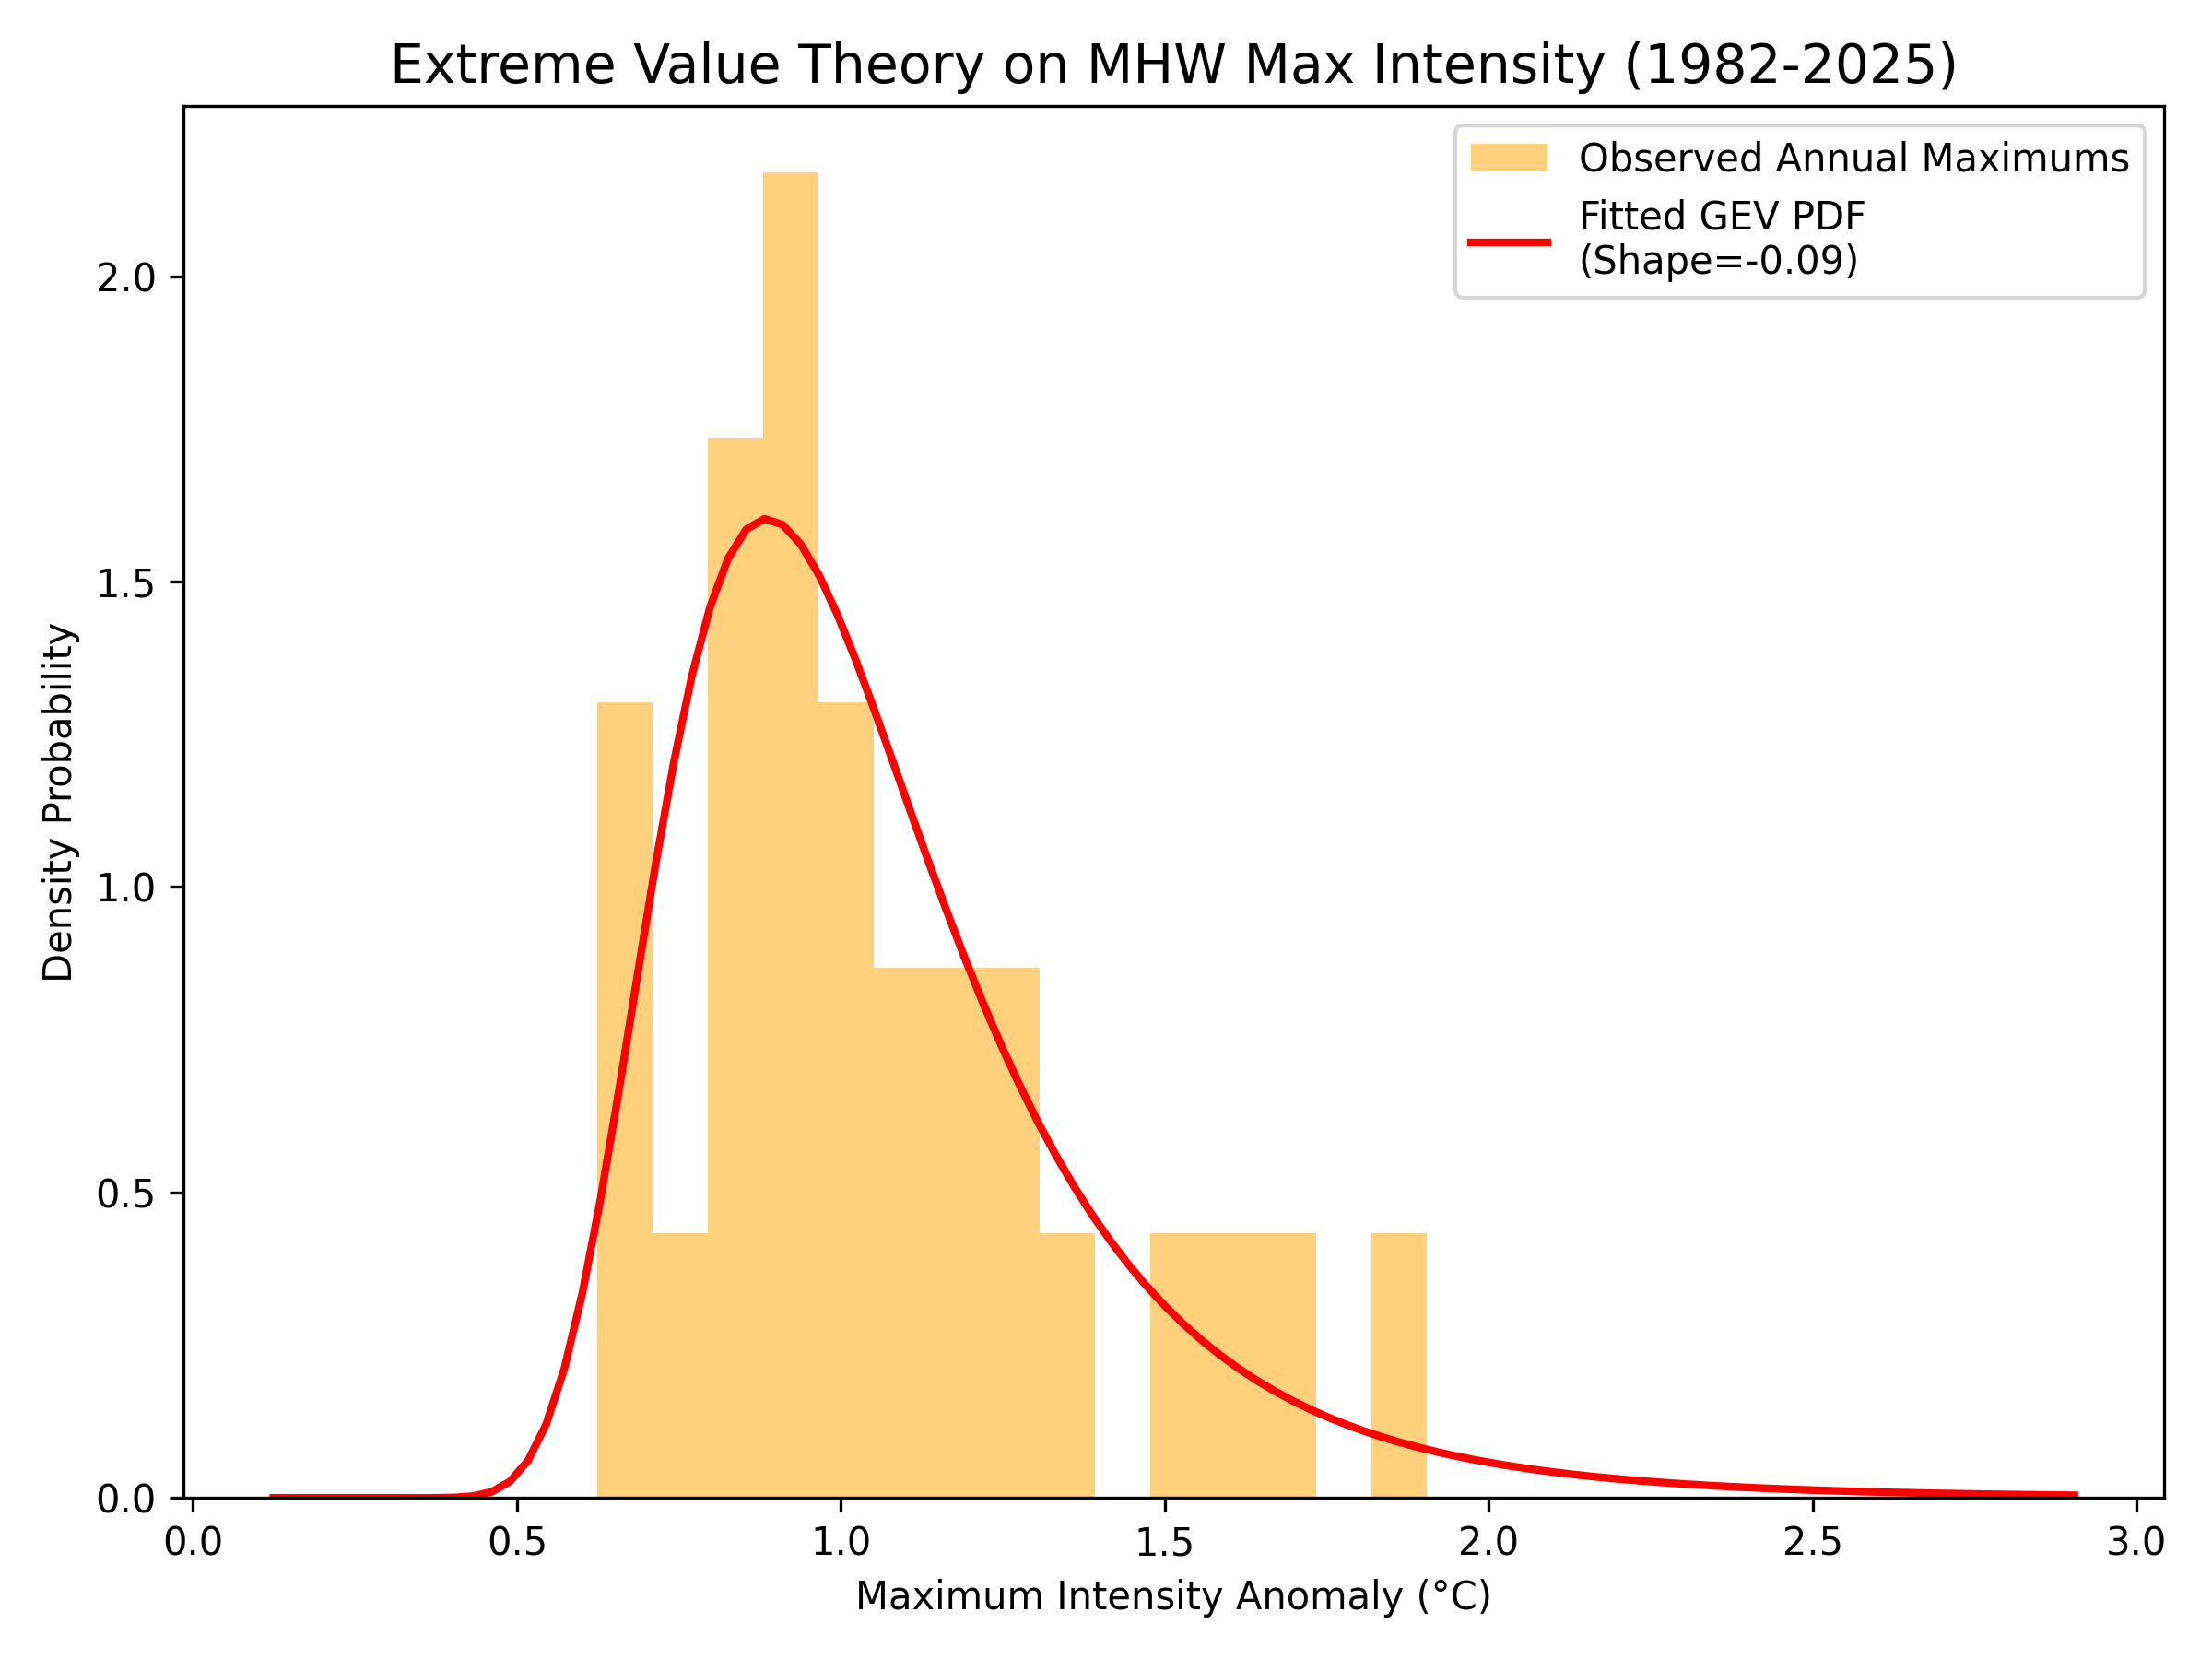
\includegraphics[width=0.75\textwidth]{../figures/evt_fit_mhw_intensity.png}
    \caption{GEV Probability Density Function fitted over the Annual Maximum MHW Intensities.}
    \label{fig:evt}
\end{figure}

Translating the fitted parameters into predictive Return Periods yields alarming baselines:
\begin{itemize}[leftmargin=1.5em]
    \item A \textbf{1-in-10 Year} Return Period event is projected to hit a +1.48$^\circ$C peak anomaly.
    \item A \textbf{1-in-50 Year} Return Period event equates to a massive +1.99$^\circ$C anomaly layer.
    \item A \textbf{1-in-100 Year} Return Period event projects to a catastrophic +2.23$^\circ$C sustained deviation against the 30-year climatology baseline.
\end{itemize}

\section{Sensitivity and Driver Composites}
The robustness of the detection metric was tested by varying the climatological window and the percentile threshold. As seen in the sensitivity analysis, while the absolute number of events scales inversely with the threshold, the most extreme events (such as the 1997 anomaly) persist across all strictness tests, proving their physical dominance rather than being an artifact of the mathematical threshold.

\begin{figure}[H]
    \centering
    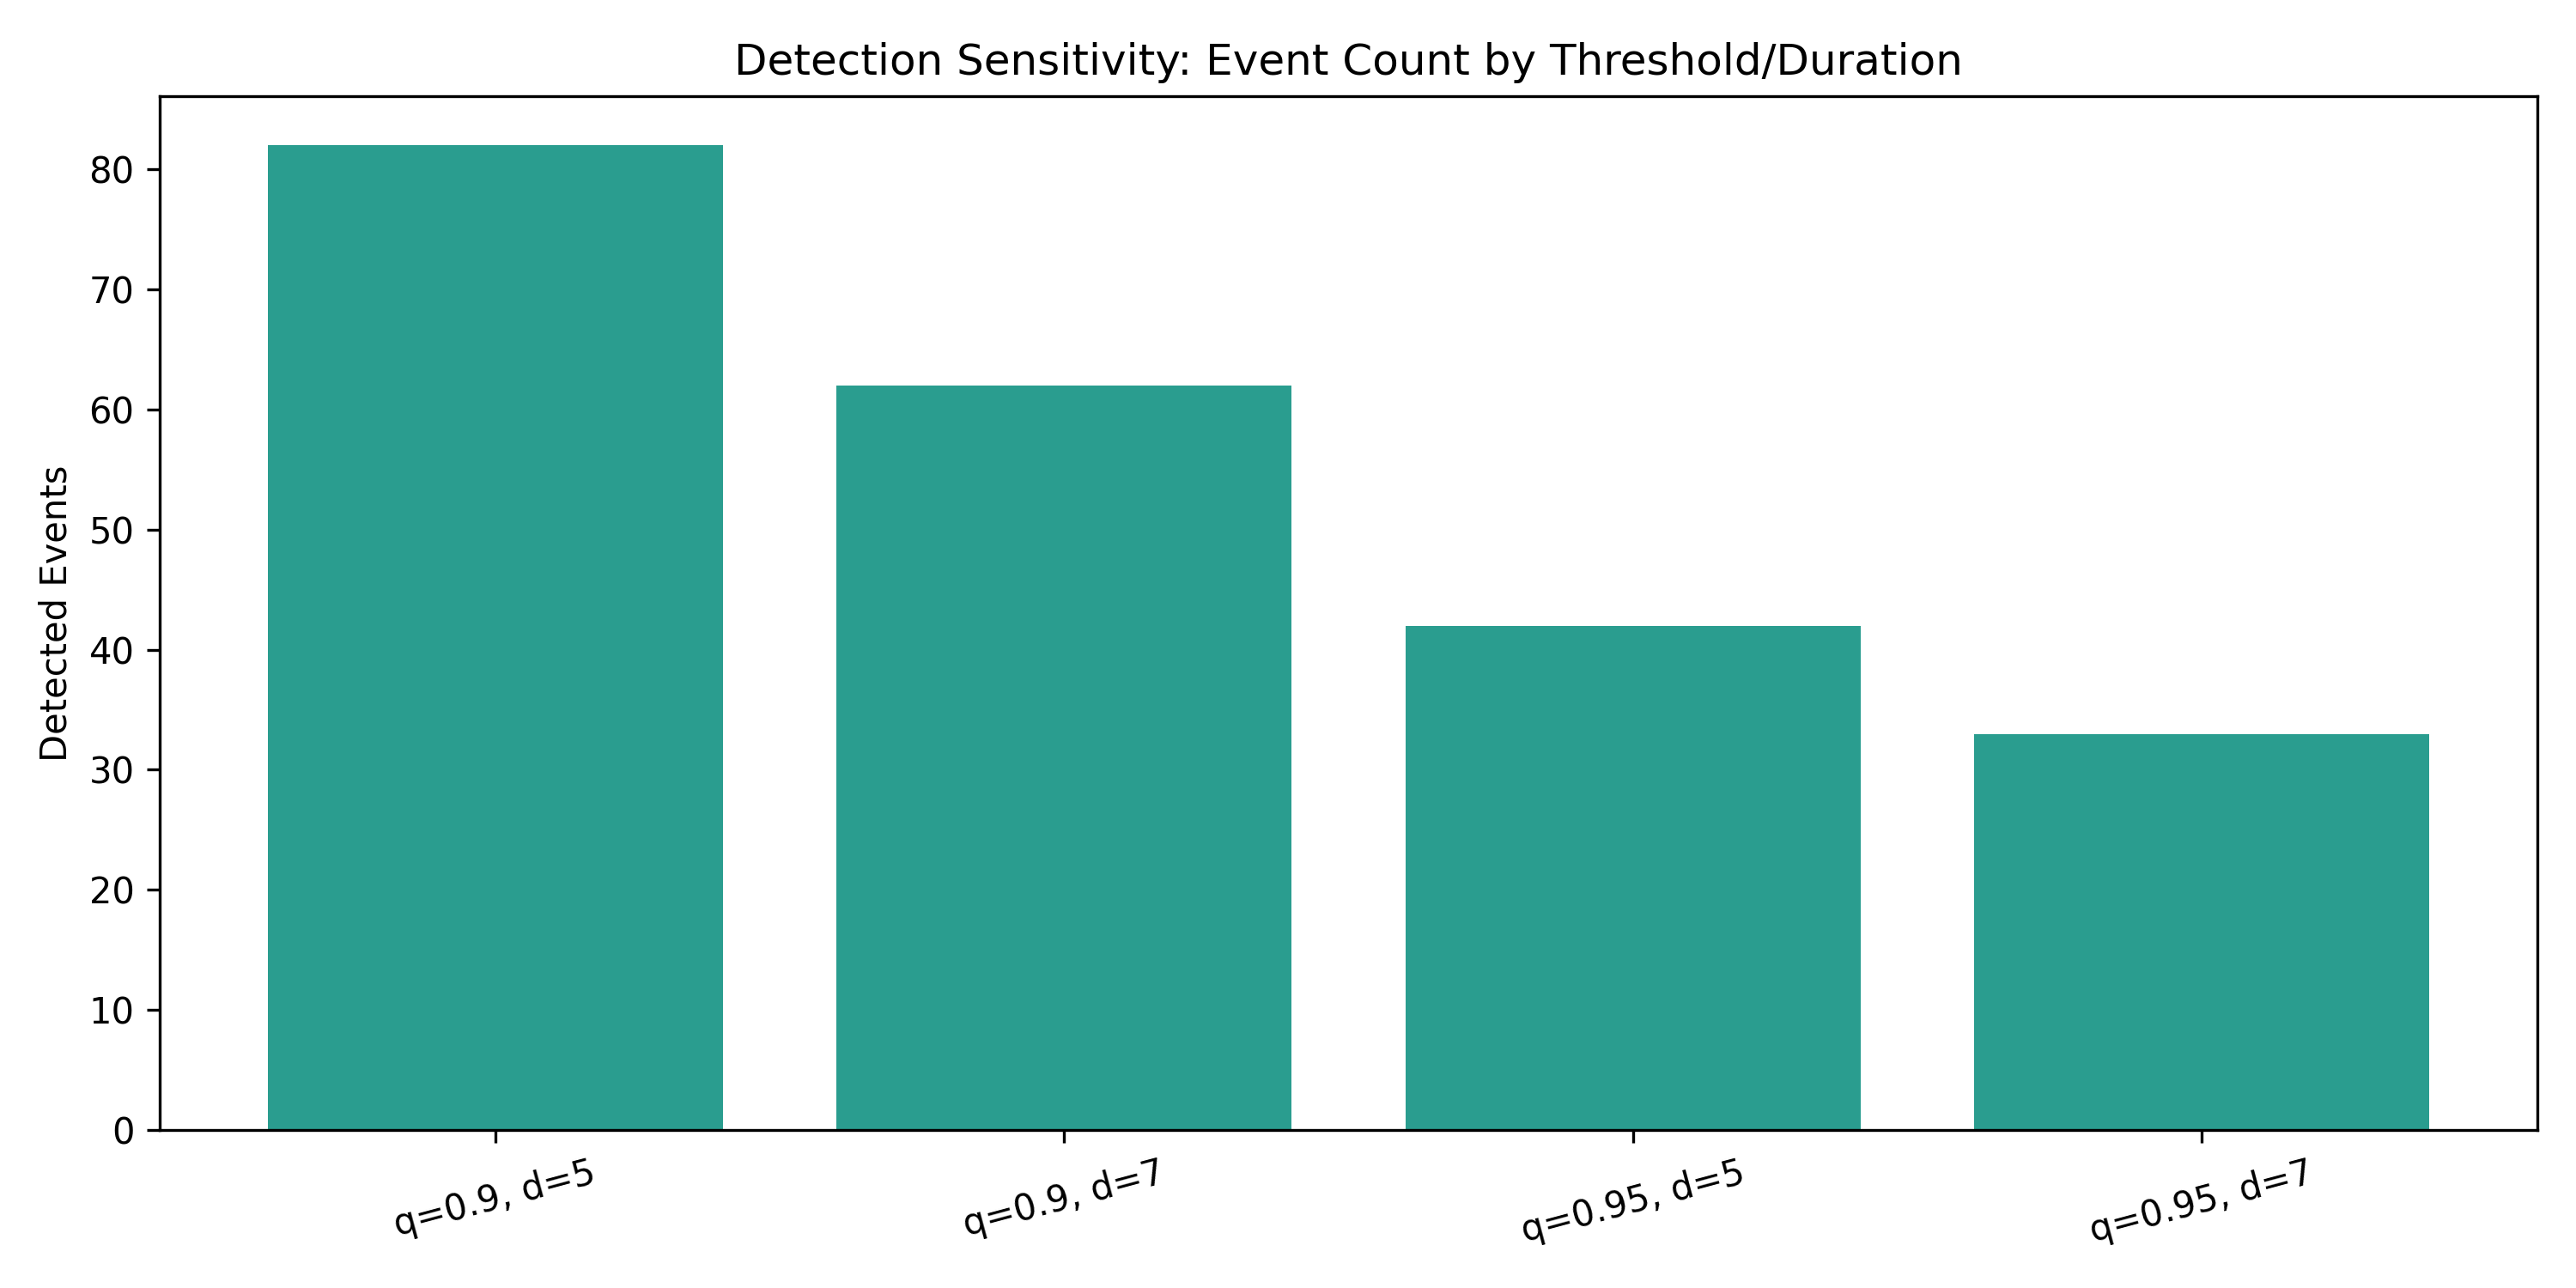
\includegraphics[width=0.6\textwidth]{../figures/sensitivity_event_count.png}
    \caption{Sensitivity Analysis showing the number of detected MHWs across varying percentile thresholds (85th to 95th) and duration minimums.}
    \label{fig:sensitivity}
\end{figure}

By examining composite profiles of external drivers (e.g. upwelling favorable winds and chlorophyll-a concentrations) aligned to the onset of a heatwave, we observe that biological productivity (chlorophyll) predictably collapses concurrently with the thermal spike.

\begin{figure}[H]
    \centering
    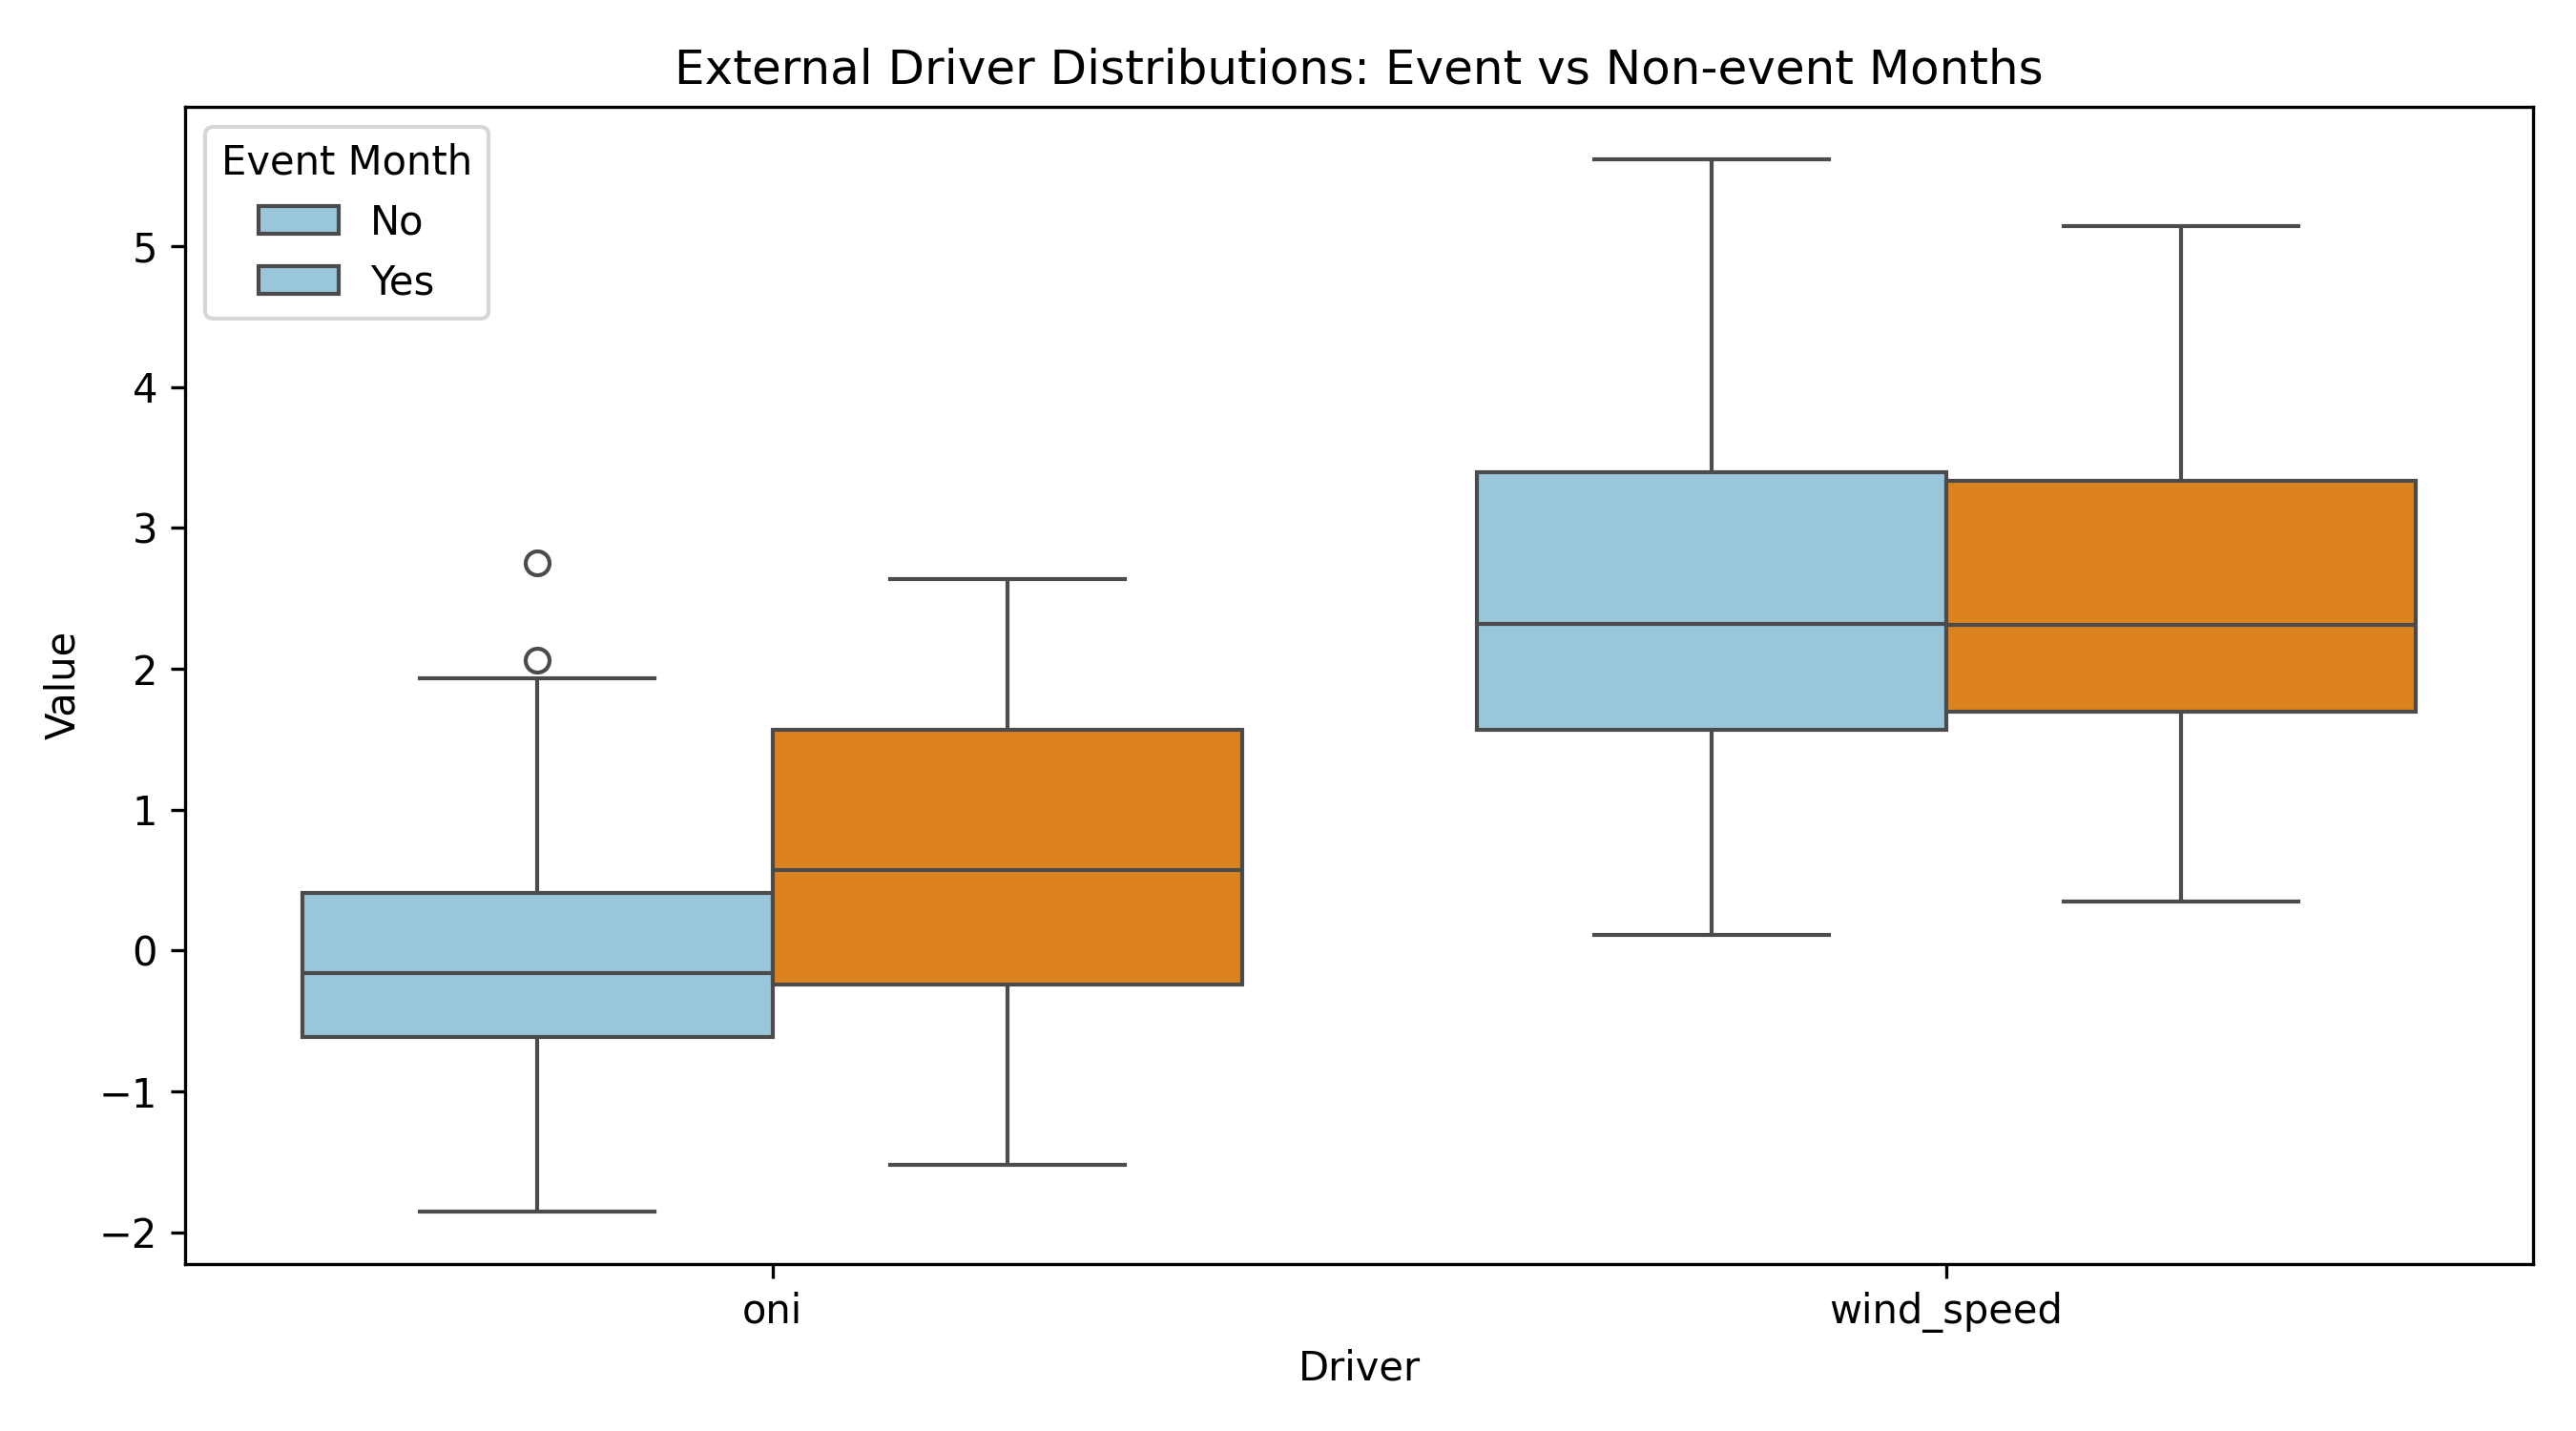
\includegraphics[width=0.85\textwidth]{../figures/driver_event_composites.png}
    \caption{Composite anomalies of associated physical drivers centered around MHW onset (Day 0).}
    \label{fig:drivers}
\end{figure}

\section{Top Historical Events Analysis}

The most catastrophic MHW burdens mathematically map to recorded strong El Niño manifestations. A ranking of the top events by cumulative intensity solidifies the 1997-1998 event as unparalleled in raw power.

\begin{table}[H]
\centering
\caption{Top 5 Most Intense Marine Heatwaves in the Humboldt Current (1982-2024)}
\begin{tabular}{llccc}
\toprule
\textbf{Start Date} & \textbf{End Date} & \textbf{Duration} & \textbf{Max Int.} & \textbf{Cum. Int.} \\
\midrule
1997-05-26 & 1998-01-03 & 223 Days & +1.90$^\circ$C & 288.87 \\
2017-01-10 & 2017-04-08 & 89 Days & +1.70$^\circ$C & 100.15 \\
1983-04-07 & 1983-08-16 & 132 Days & +1.60$^\circ$C & 147.64 \\
2023-06-04 & 2023-11-11 & 161 Days & +1.56$^\circ$C & 186.44 \\
2023-02-04 & 2023-06-02 & 119 Days & +1.48$^\circ$C & 118.58 \\
\bottomrule
\end{tabular}
\end{table}

\subsection{Case Study: The 1997-1998 "Godzilla" El Niño}
The 1997-1998 event stands as a paradigm-defining occurrence. By isolating the daily SST against the climatology and the 90th percentile threshold, the true magnitude of this event becomes apparent.

\begin{figure}[H]
    \centering
    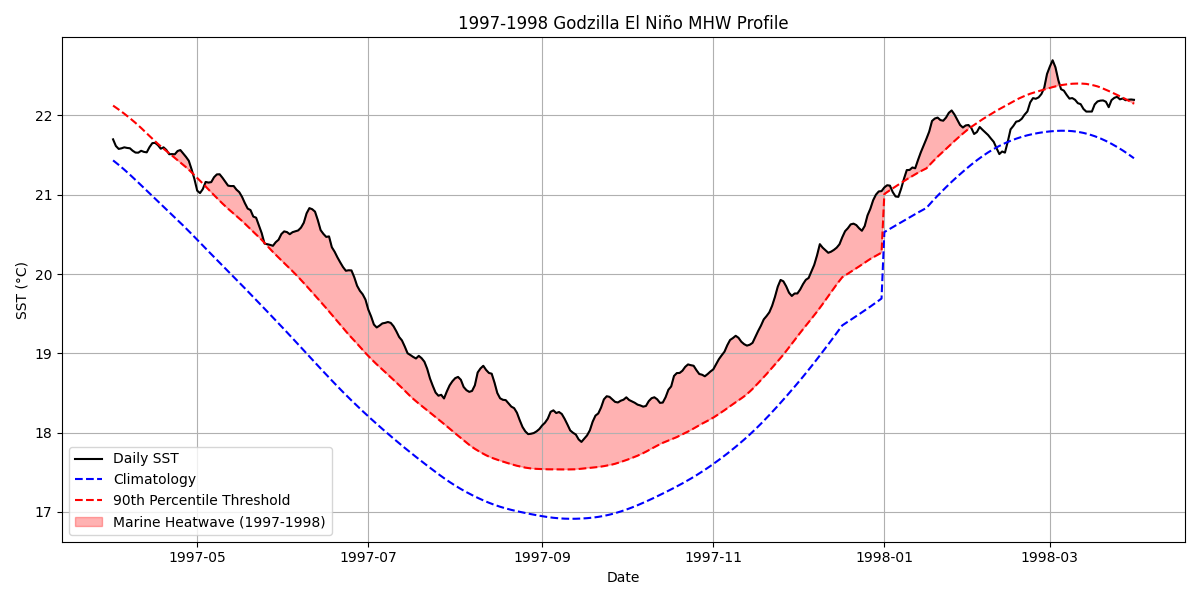
\includegraphics[width=1.0\textwidth]{../figures/event_1997_profile.png}
    \caption{Daily SST profile of the 1997-1998 Marine Heatwave. The persistent red shading indicates the continuous period where SST exceeded the localized 90th percentile threshold, showcasing an unrelenting thermal stress lasting over 200 days.}
    \label{fig:event_1997}
\end{figure}

During this event, the Humboldt Current experienced an unprecedented collapse of its upwelling system, with surface temperatures consistently exceeding the threshold for nearly 8 consecutive months. The biological ramifications were severe, resulting in the massive displacement of the anchoveta population and widespread seabird mortality. The sheer unbroken duration of this anomaly underscores the vulnerability of coastal systems to macro-basin forcing.

\section{Discussion}
This research differentiates the Humboldt dynamics from those observed in Indian Ocean basins (such as the Arabian Sea). While those regions are heavily regulated by monsoonal shifts and basin-scale atmospheric heat blankets, Humboldt anomalies are intrinsically oceanic, propelled horizontally by equatorial Kelvin waves and vertical stratification. The PCA findings confirm that nearly half the temperature variance along the coast is dictated directly by this ENSO connection, leaving local upwelling regimes largely at the mercy of equatorial winds thousands of kilometers away.

Furthermore, the STL decomposition and Mann-Kendall statistics prove an underlying continuous warming trend independent of ENSO cycles. 

\section{Conclusion}
This study shifts the analytical lens away from dashboard-based forecasting toward rigorous structural and physical oceanographic characterization. By implementing daily-resolution detection metrics, the research exposes a system whose extreme warming behavior is governed less by subtle, progressive baseline shifts, and more by chaotic, large-scale climatic forcing signatures effectively captured via EOF spatial decomposition. The 100-year return period projections reaching +2.23$^\circ$C warn of dire consequences for the EBUS ecosystem if global mitigation falters. These findings reaffirm that coastal ecosystem fragility in Eastern Boundary systems requires event-scale interannual decomposition, extending beyond generic continuous-state predictability workflows. 

\begin{thebibliography}{9}

\bibitem{hobday2016}
Hobday, A. J., Alexander, L. V., Perkins, S. E., et al. (2016).
\textit{A hierarchical approach to defining marine heatwaves}.
Progress in Oceanography, 141, 227-238.

\bibitem{hobday2018}
Hobday, A. J., Oliver, E. C., Sen Gupta, A., et al. (2018).
\textit{Categorizing and naming marine heatwaves}.
Oceanography, 31(2), 162-173.

\bibitem{oliver2018}
Oliver, E. C., Donat, M. G., Burrows, M. T., et al. (2018).
\textit{Longer and more frequent marine heatwaves over the past century}.
Nature communications, 9(1), 1-12.

\bibitem{sydeman2014}
Sydeman, W. J., Garcia-Reyes, M., Schoeman, D. S., et al. (2014).
\textit{Climate change and wind intensification in coastal upwelling ecosystems}.
Science, 345(6192), 77-80.

\bibitem{oisst21}
Huang, B., Liu, C., Banzon, V., et al. (2021).
\textit{Improvements of the Daily Optimum Interpolation Sea Surface Temperature (DOISST) Version 2.1}.
Journal of Climate, 34(8), 2923-2939.

\end{thebibliography}

\end{document}